\chapter{Results}\label{chap:results}

\ifpdf
    \graphicspath{{results/figs/Raster/}{results/figs/PDF/}{results/figs/}}
\else
    \graphicspath{{results/figs/Vector/}{results/figs/}}
\fi

\epigraph{Hold on. This whole operation was your idea.}{Anakin Skywalker}

Now that we are caught up with the technical logistics of the instrument as well as the mathematical prescription to calibrate it, we assess the capabilities of our method under the scrutiny of varied sets of data. Throughout the process of our research, practical development of the receiver reformed our approach to calibration which consequently reshaped the implementation of our instrument design. In the continuous interchange of physical and mathematical adjustments, a great deal of experiments were undertaken to increase the potency of our algorithm, often to little or no effect. The results presented here demonstrate the incremental progress in calibration accuracy up to the time of deployment in the Fall of 2023. We start by briefly detailing the application of data taken before construction of the REACH receiver as a proof-of-concept that reasonable calibrated temperatures can be retrieved. Following this, we give results from the application of simulated data to assess the noise floor of our algorithm under idealised conditions. We then exhibit the capabilities of our algorithm using laboratory data taken from a partially-constructed REACH receiver as well as a HERA receiver to demonstrate the further application of the procedure to other experiments. Results from data collected with a completed REACH receiver are shown along with an overview of attempts to increase the effectiveness of our technique through physical and computational adjustments. We then compare our results to the conventional formulation as a sanity check before discussing efforts with more advanced methods after which we appraise the state of the field considering these developments.


% =========================================
\section{Preliminary laboratory measurements}\label{sec:mphil_results}
Whilst construction of the receiver was underway, preliminary experiments were performed to gauge the performance of our calibration procedure. An initial dataset was produced using some of the publicly available EDGES data and laboratory measurements taken at Cambridge using various disconnected instruments. Two calibration sources were used for our measurements; a $50 \Omega$ load at ambient temperature and a heated source constructed from a $50 \Omega$ load coupled to a ThermOptics DN511 proportional heater set to 373 K and attached to a 4-inch rigid coaxial cable similar to the apparatus detailed in \cref{sec:frontend}. Temperatures for these calibration sources were assumed to be 298 K and 373 K respectively and were not measured during the experiment.

As the receiver was not yet built, a Dicke switch was approximated by manually swapping sources at the front of the signal chain. An additional $50 \Omega$ load was used as the reference load while a Noisecom NC346A noise diode with 5 dB of attenuation was used as the reference noise source. The Noisecom NC346A was chosen for its stable noise output value of $\sim 350$ K over the frequency band of interest as shown in TABLE and resembling the specifications of the internal reference noise source used by the EDGES team. Reflection data for the devices was taken using the Keysight N5247A PNA-X VNA. An RF signal chain was created for PSD measurements which consisted of 10 metres of coaxial cabling preceding a custom built LNA with specifications shown in \cref{tab:mphil_lna}. Following the LNA, the signal was filtered before reaching a CASPER ROACH-2 ADC/spectrometer made from an AMD XILINX Virtex-6 FPGA.

Combining our measurements of the ambient and heated loads along with the noise wave parameters published by EDGES ($\T{unc}$, $\T{cos}$, $\T{sin}$, $C_1$ and $C_2$), a system of calibration equations was established in which the noise temperatures for the internal reference load and noise source were calculated under their model and plotted in \cref{fig:mphil_result} as the red and dark blue data respectively. Returning to our formulation as specified in \cref{sec:formalism} MAKE SURE REFER TO OUR FOMALISM NOT EDGES, measured reflection coefficients, PSDs and the assumed temperatures were inputted into our model to solve for the noise wave parameters. 1000 posterior samples of $\T{NS}$ and $\T{L}$\footnote{now proper noise wave parameters in this formulation} from our Bayesian model are plotted in \cref{fig:mphil_result} in orange and cyan respectively.
\begin{figure}
    \centering
    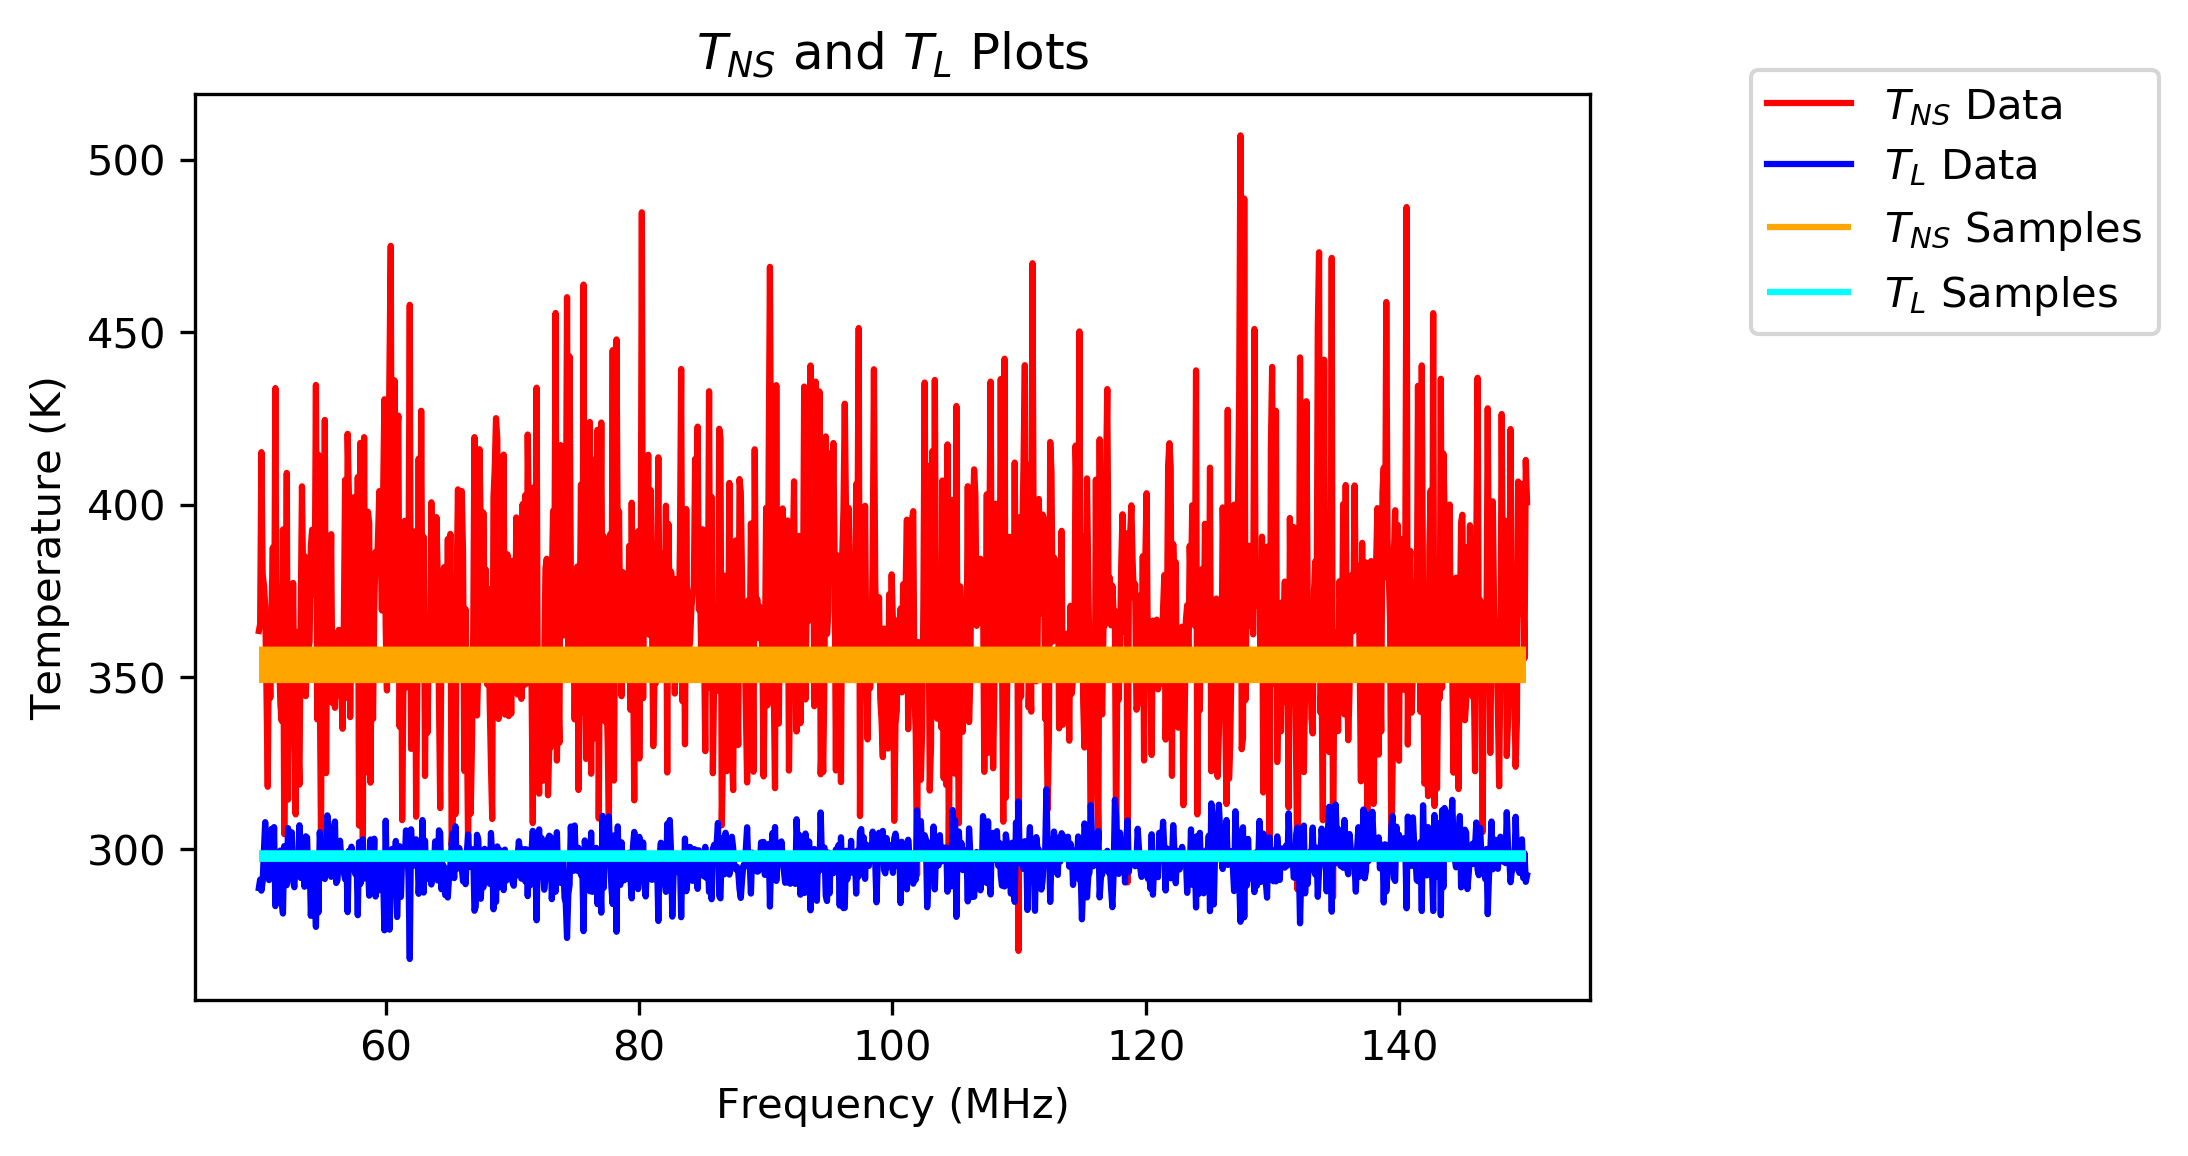
\includegraphics[width=.8\textwidth]{mphil_result}
    \caption{Calculations of $\T{NS}$ and $\T{L}$ from initial datasets taken before construction of the REACH receiver. Two-minute integrations and reflection coefficient data were taken of the ambient and heated $50 \Omega$ loads. The red and dark blue show the resulting $\T{NS}$ and $\T{L}$ from solving a linear set of calibration equations under the EDGES formulation for calibratin a receiver. The orange and cyan show 1000 posterior samples for $\T{NS}$ and $\T{L}$ from our Bayesian algorithm. The agreement between the system-of-equations and Bayesian solutions indicates the validity of our changes to the formulation. Recovery of the assumed noise temperatures of the internal reference noise source and load (350 K and 300 K respectively) shows that noise wave parameter values may be determined under our Bayesian algorithm. Finally, the reduction of noise apparent in the Bayesian solution is encouraging suggests that the method improves calibration accuracy.}
    \label{fig:mphil_result}
\end{figure}

The apparent agreement between the system solution and our Bayesian model supports our assertion that the absorption of the EDGES $C_1$ and $C_2$ parameters into an effective $\T{NS}$ and $\T{L}$ is a valid procedure. Furthermore, recovery of the internal reference noise temperatures assumed by EDGES, 350 K and 300 K for the internal noise source and load respectively, shows that our model can correctly determine the $\T{NS}$ and $\T{L}$ parameters using ambient and heated source data. Additionally, the reduction of noise in the Bayesian solution suggests that our method improves calibration accuracy when subjected to identical data. 


% =========================================
\section{Results with simulated data}\label{sec:simulated_data}
To verify the performance of our pipeline and highlight features of the algorithm, we evaluate the results of self-consistency checks using empirical models of data based on measurements taken in the laboratory. To make this data as realistic as possible, we used actual measurements of the reflection coefficients of many types of calibrators (see \cref{tab:sim_calibrators}) to generate power spectral densities using \cref{eqn:pant,eqn:pl,eqn:pns} given a set of realistic model noise wave parameters along with some assumptions about the noise, which are described in REFER TO THE SECTION WHERE WE DESCRIBE ADDING NOISE TO THE SIMULATED CALIBRATORS. The impedance of the calibrators which were measured with a vector network analyser (VNA) and used in our pipeline are shown on a Smith chart in \cref{fig:sim_data_smith}
\begin{table}
    \centering
    \begin{tabular}{lcc}
    \hline
    Calibrator & Temperature\\
    \hline
    Cold load ($50 \ \Omega$) & 298 K\\
    Hot load ($50 \ \Omega$) & 373 K\\
    Gore cable $+ 5 \ \Omega$ & 298 K\\
    Gore cable $+ 500 \ \Omega$ & 298 K\\
    Gore cable $+ 31 \ \Omega$ & 298 K\\
    Gore cable $+ 81 \ \Omega$ & 298 K\\
    $25 \ \Omega$ resistor & 298 K\\
    $100 \ \Omega$ resistor & 298 K\\
    \hline
    \end{tabular}
    \caption{Table of calibrators used in the creation of our empirical data models for analysis. Calibrators were inputted in pairs in the order shown when demonstrating the effects of additional calibrator information (see REFER TO SECTION ON INCREASING CALIBRATOR NUMBER).}
    \label{tab:sim_calibrators}
\end{table}

\begin{figure}
    \centering
    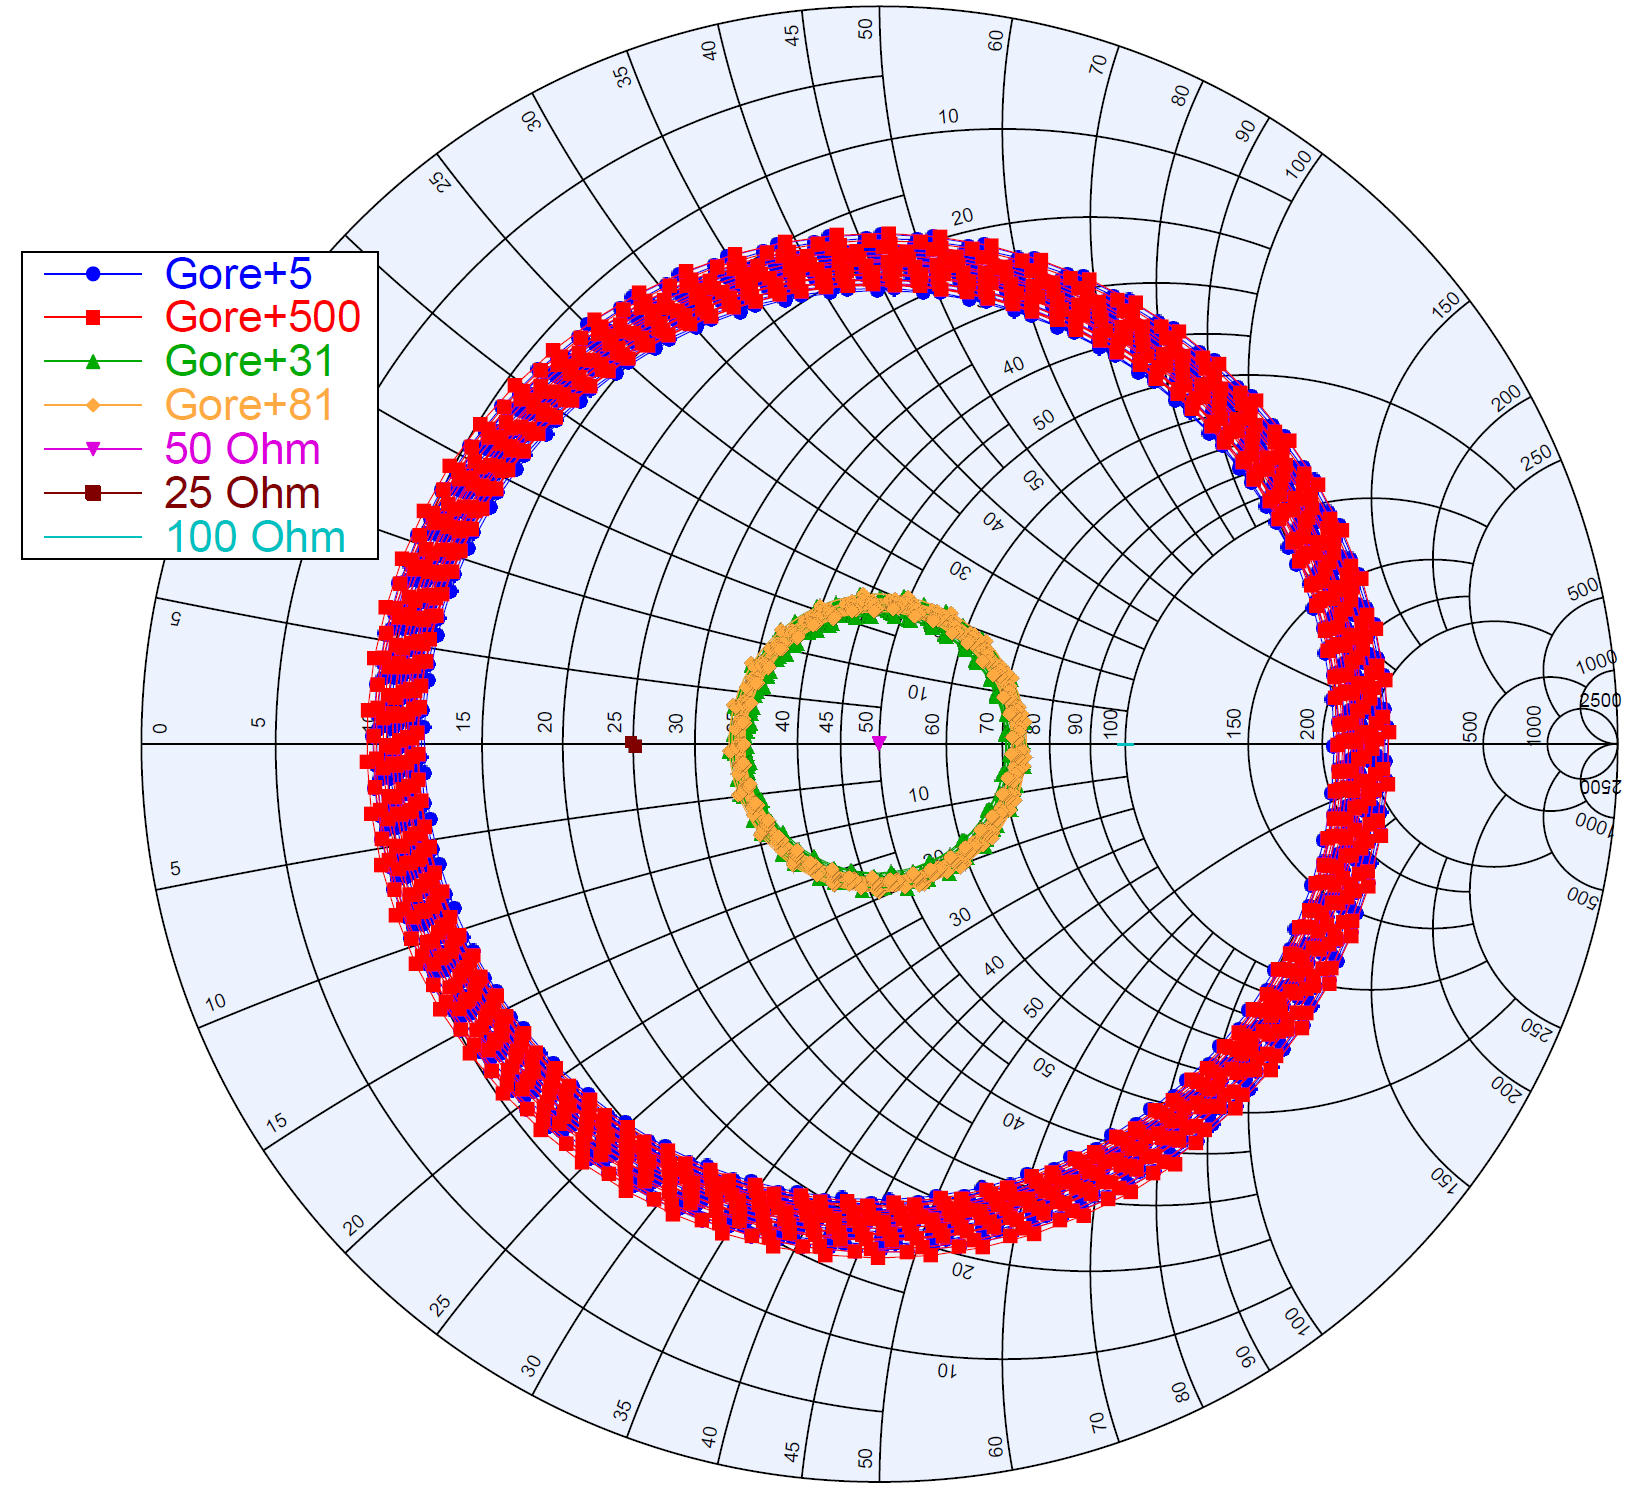
\includegraphics[width=.5\columnwidth]{sim_data_smith}
    \caption{Smith chart showing the measured complex impedance of devices used to create empirical models of calibration sources for testing of our Bayesian algorithm.
    \label{fig:sim_data_smith}}
\end{figure}

We start by demonstrating the importance of correlation between noise wave parameters when determining their values to provide a better calibration solution (\cref{sec:correlation}). We then show the increased constraints on these noise wave parameters attributed to the inclusion of more calibrators than the standard number of four (REFER TO SECTION). Following this, we illustrate the effectiveness of model selection for the optimisation of individual noise wave parameters to prevent the loss of information resulting from overfitting or underfitting of the data (REFER TO SECTION). Finally, these features are incorporated into a calibration solution applied to a $50 \ \Omega$ load (REFER TO SECTION).


% =========================================
\subsection{Correlation between noise wave parameters}\label{sec:correlation}
The first major feature of our Bayesian pipeline is the consideration of possible correlation between noise wave parameters when deriving their values. This is best demonstrated when noise is introduced in an idealised way as to retain a form matching the Gaussian form of our mathematical model. To do this, empirical models of power spectral densities are calculated from \cref{eqn:pant,eqn:pl,eqn:pns} using measurements of $\G{rec}$, $\Ga$ and $\T{cal}$ for the cold and hot loads, as well as a set of realistic fiducial noise wave parameters. Gaussian noise of one unit variation is then added to the $\T{cal}$ measurements after the calculation to conserve its Gaussian form. This data is submitted to our algorithm and the resulting posterior distributions for coefficients of the polynomial noise wave parameters are compared to the fiducial values.

Such posterior distributions can be seen in \cref{fig:goodplot} showing the results of models using only the cold load (grey posterior), only the hot load (red posterior) and using both loads in tandem (blue posterior). For these calculations we chose a set of model noise wave parameters as constants across the frequency band;
\begin{align*}
    & \T{unc} = 250 \ \mathrm{K} \\
    & \T{cos} = 190 \ \mathrm{K} \\
    & \T{sin} = 90 \ \mathrm{K} \\
    & \T{NS} = 1200 \ \mathrm{K} \\
    & \T{L} = 298 \ \mathrm{K}
\end{align*}

In \cref{fig:goodplot}, a strong correlation between the $\T{L}$ and $\T{NS}$ is evident as the hot-load posterior is highly skewed as expected from \cref{eqn:xl,eqn:xns}. The resulting intersection of posteriors from the individual loads facilitate the derivation of noise wave parameters as the dual-load posterior is found within the region of posterior overlap crossing with the values of the model shown in the inset of \cref{fig:goodplot}. Retrieval of the noise wave parameter values using correlations between them found in the data demonstrate the relevance of this information which is not taken into account in previous calibration techniques.
\begin{figure}
    \centering
    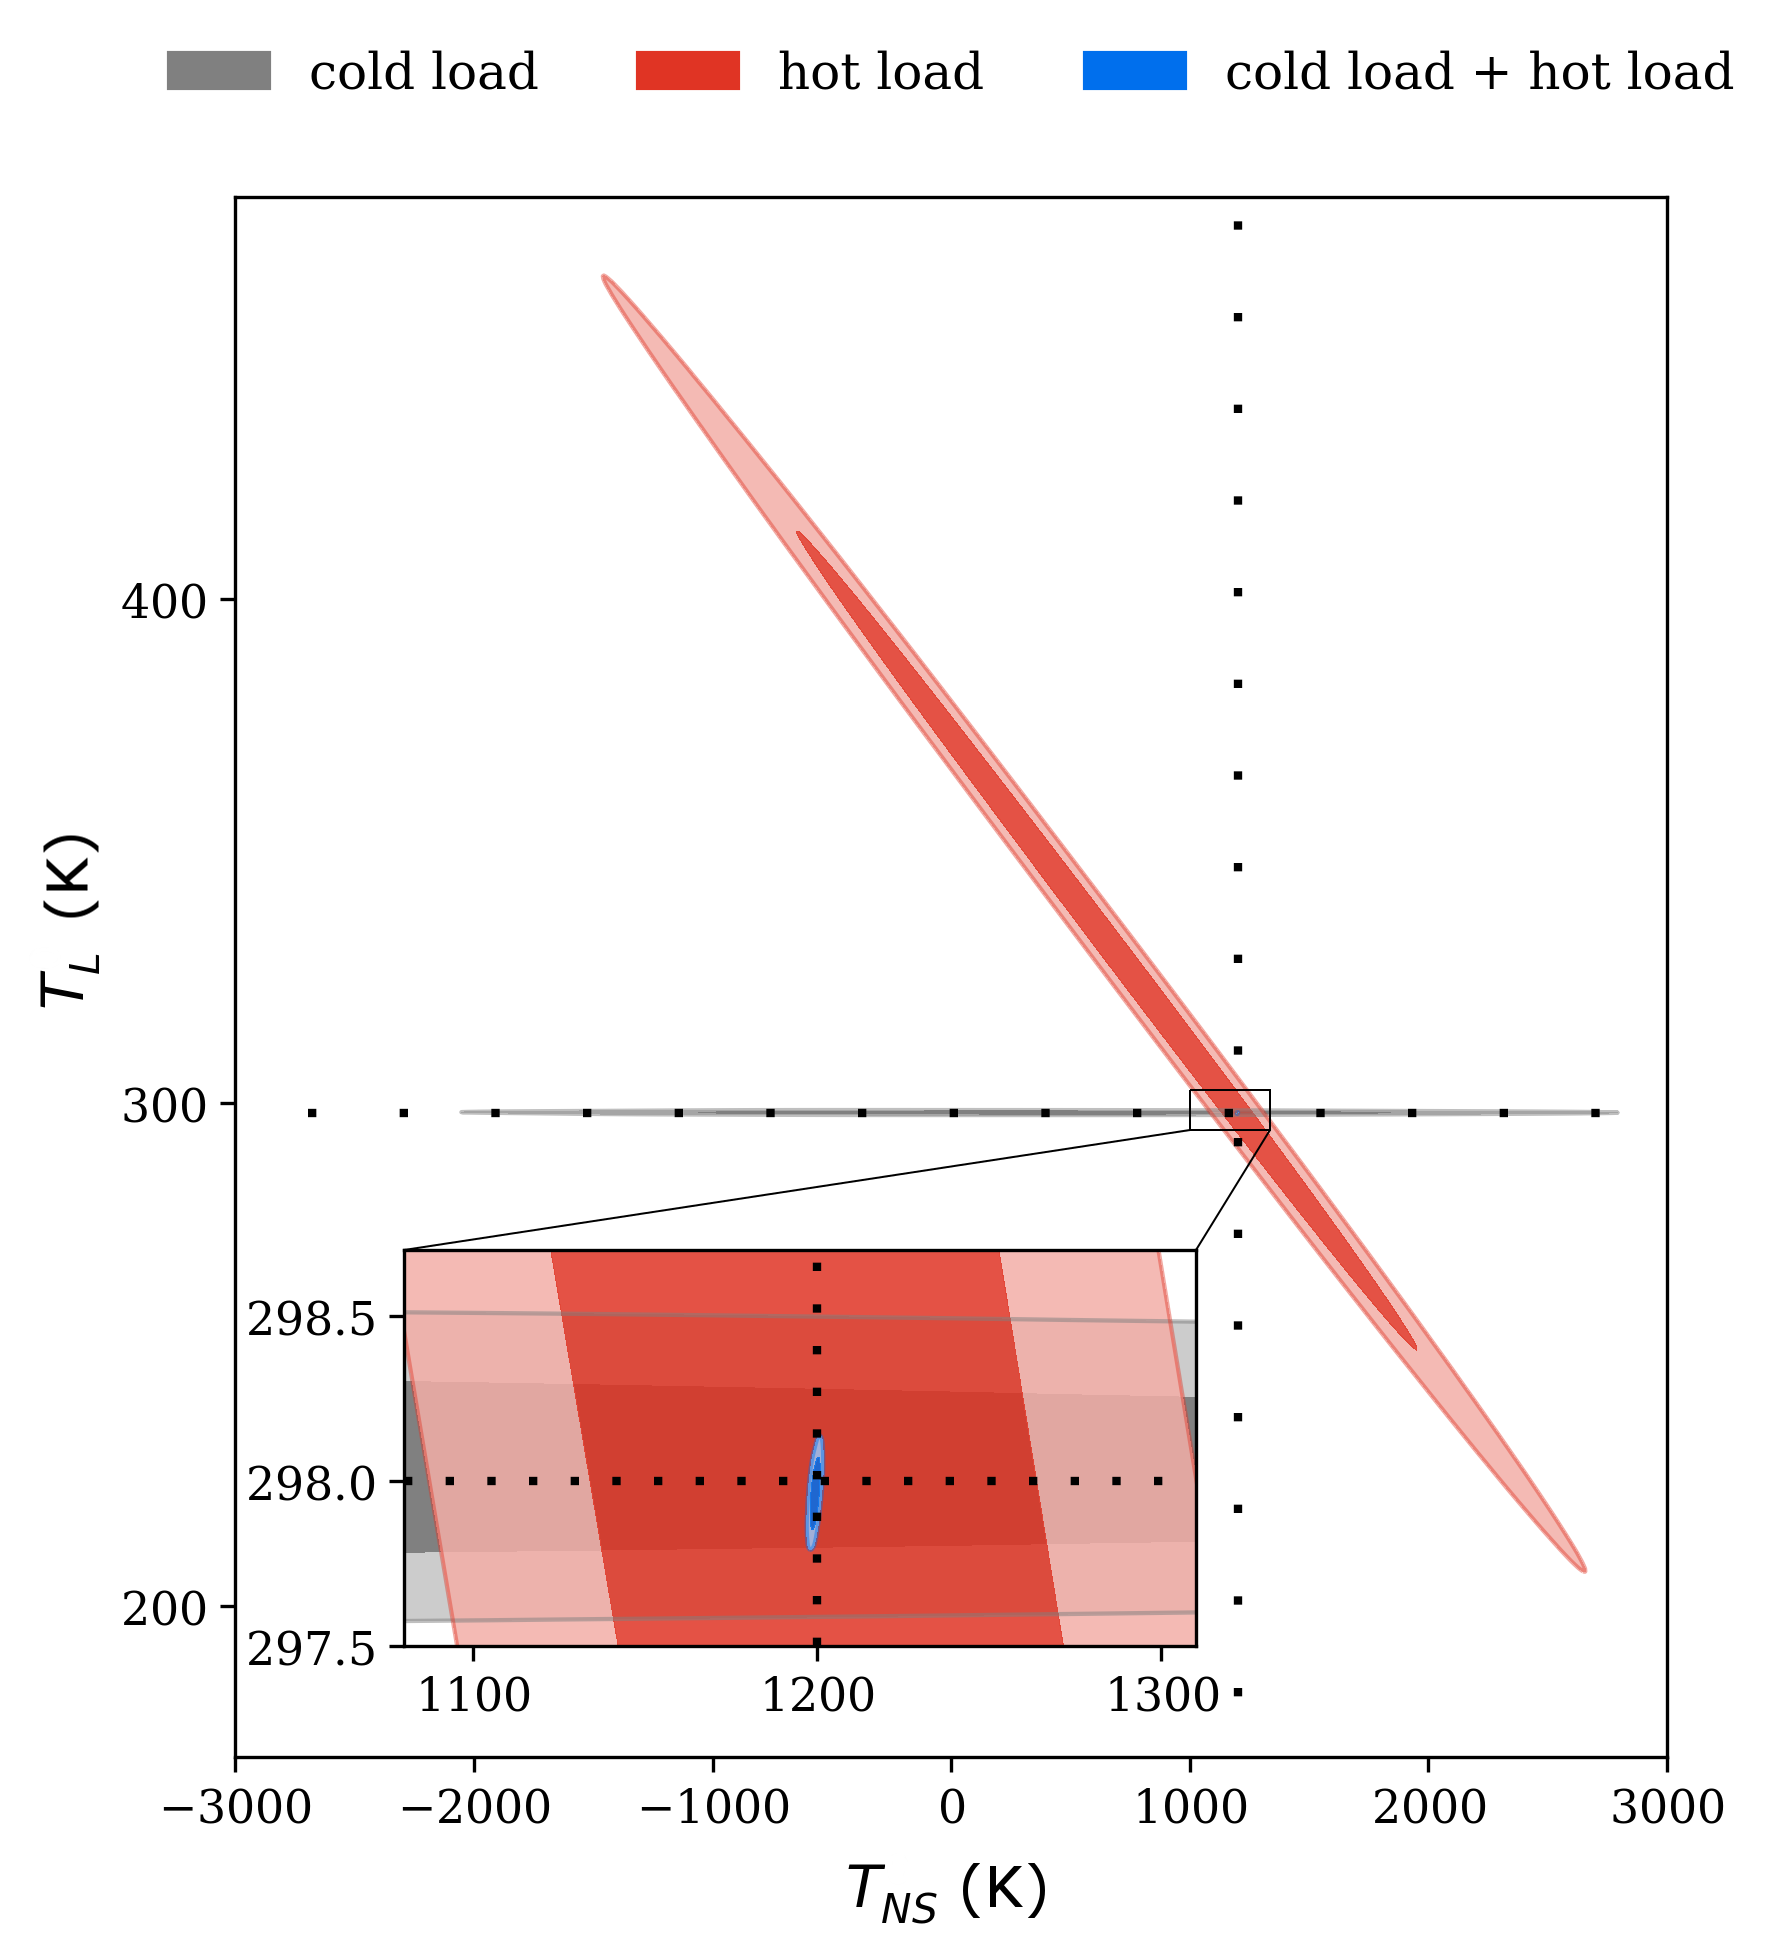
\includegraphics[width=.5\columnwidth]{goodplot}
    \caption{Plot showing the joint posteriors of $\T{L}$ and $\T{NS}$ for models using the cold load, the hot load, and both loads concurrently shown as the grey, red and blue posteriors respectively. The black cross hairs mark the noise wave parameter values used to generate data submitted to the pipeline. A zoom-in of the posterior intersection is provided to illustrate the constraint of noise wave parameter values attributed to the correlation between parameters. \label{fig:goodplot}}
\end{figure}


% =========================================
\subsection{Constraints with additional calibrators}\label{sec:multCal}
Another feature of our pipeline is the ability to include as many calibrators as required to constrain the calibration parameters. For analysis, six more calibrators are introduced in pairs following the order presented in \cref{tab:sim_calibrators}. We include data generated from measurements of multiple resistors terminating a high quality 25 m cable made by GORE\textsuperscript \textregistered\footnote{At this stage of development, we had not decided on which model of cable would optimise both calibration results and cost efficiency. While we eventually chose the LMC195 cabling detailed in \cref{sec:frontend}, many early datasets included the high quality, but expensive GORE\textsuperscript \textregistered cabling.}.  Data for these calibrators is once again generated using fixed terms and Gaussian noise of one unit variation added to $\T{cal}$ as discussed above. \Cref{fig:linearall} shows the results of models using four, six, and eight calibrators.

\begin{figure}
  \centering
  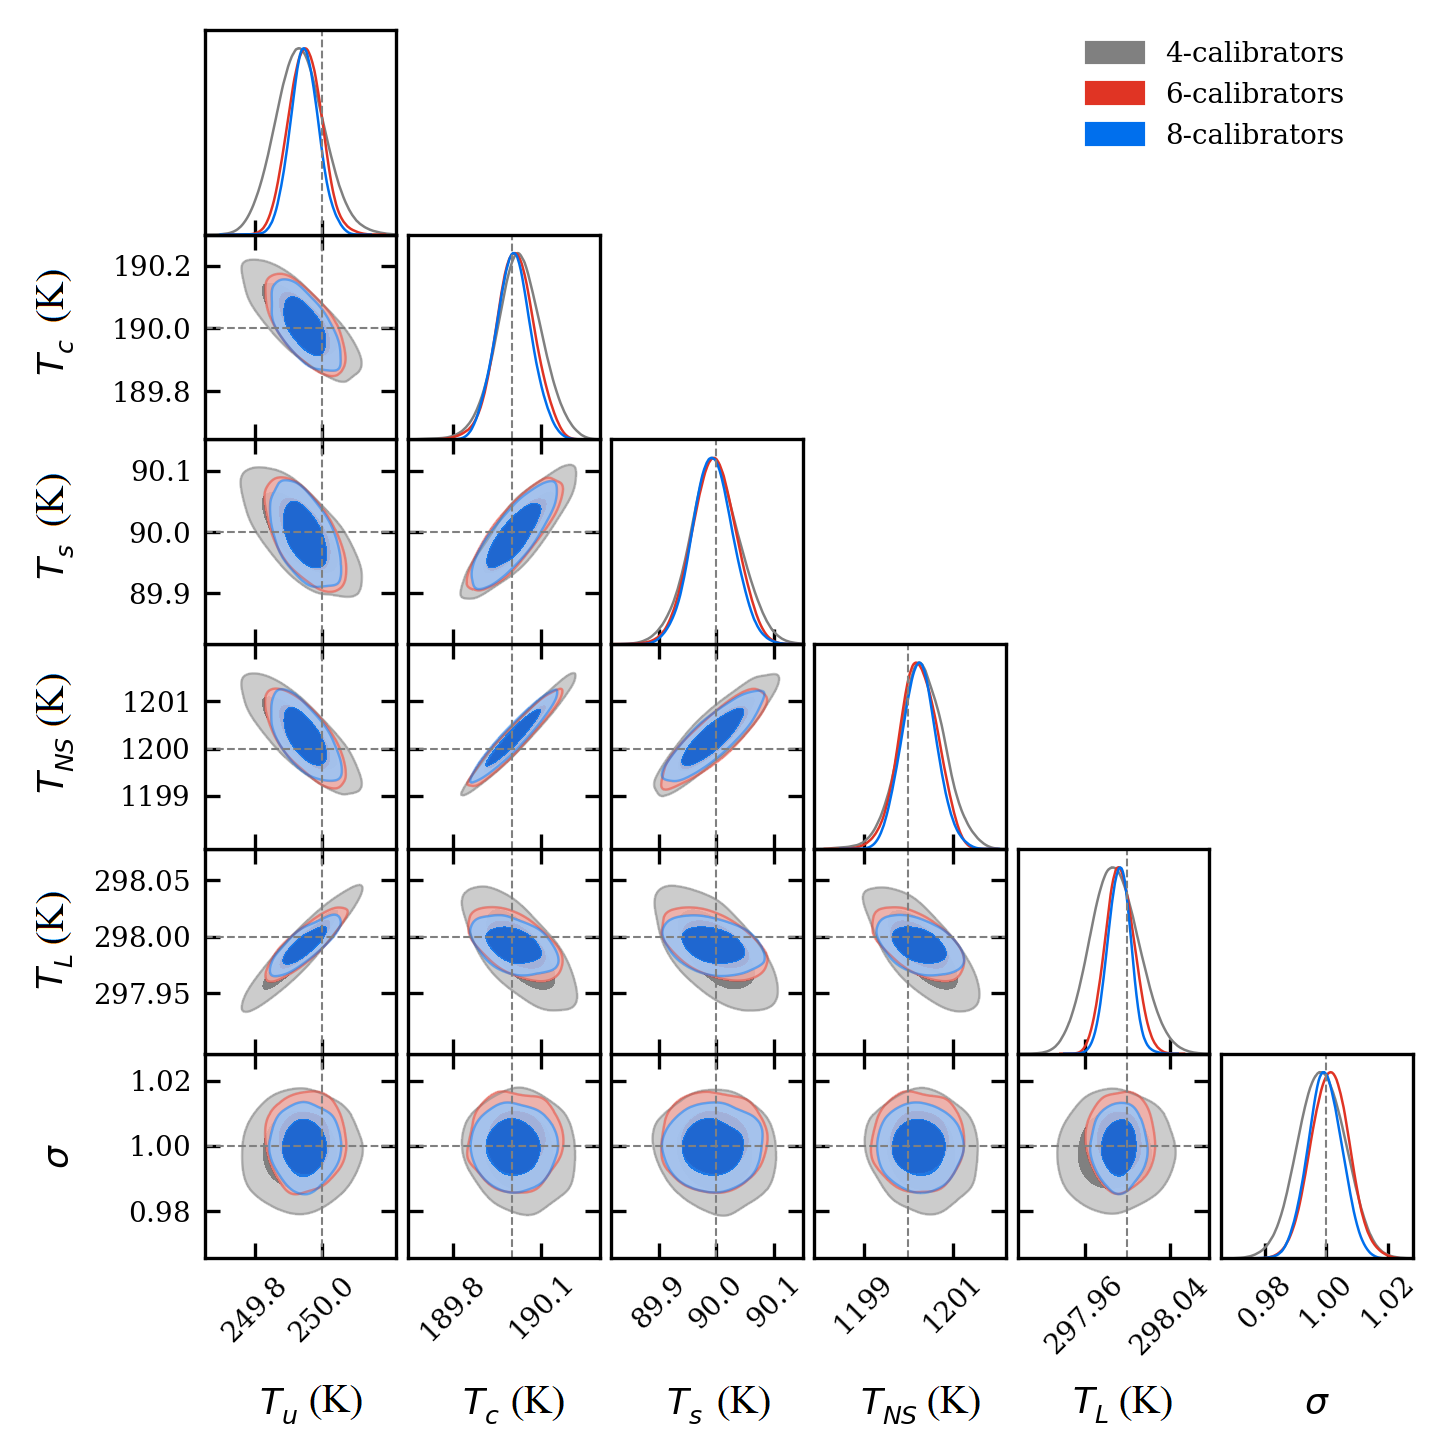
\includegraphics[width=\columnwidth]{linearall}
  \caption{Posterior results of our pipeline using data from four, six and eight calibrators shown in grey, red and blue, respectively. Cross hairs mark the values of noise wave parameters used to generate the data. These values fall within $1\sigma$ of the posterior mean values. We can see that the constraint on noise wave parameter values increases with the number of calibrators used in our pipeline which is encouraging. \label{fig:linearall}}
\end{figure}

As shown, the inclusion of more calibrators increases the constraint on the resulting noise wave parameters. However, we note that after the inclusion of four calibrators, the relative additional constraint decreases with each additional calibrator and thus the use of a large number of calibrators would be unnecessary. The values of noise wave parameters used to generate the data as indicated by the cross hairs in \cref{fig:linearall} all fall within $1\sigma$ of our pipeline's resulting posterior averages for models using all eight calibrators.


% =========================================
\subsection{Optimisation of individual noise wave parameters}\label{sec:opt}
The final highlight of our Bayesian pipeline is a use of machine learning techniques to optimise individual noise wave parameters. This is advantageous as a blanket prescription of order-seven polynomials applied to all noise wave parameters, such as done in the EDGES experiment, may underfit or overfit individual parameters and misidentify systematics or information about the signal being measured.

The optimisation procedure compares the evidences (\cref{eqn:ev}) of different models to determine the vector of noise wave parameter polynomial coefficients $\mathbfit{n}$ that best describes the data as briefly mentioned at the end of \cref{sec:bayes}. Since the model favoured by the data will have the highest evidence, we use a steepest descent procedure to compare models in `$\mathbfit{n}$-space' and determine the direction of the gradient in `evidence-space'. After multiple iterations, this brings us to the model with the maximal evidence. Since $\mathbfit{n}$ consists of five numbers corresponding to the number of polynomial coefficients for each of the five noise wave parameters, models are generated by individually increasing each index of $\mathbfit{n}$ by 1. We expect the evidence to follow an `Occam's cliff,' in which the evidence sharply increases preceding the optimal $\mathbfit{n}$ with a slow fall-off following the maximum.

To demonstrate this, data is generated using measurements from all eight calibrators of \cref{tab:sim_calibrators} and noise wave parameters as second-order polynomials
\begin{align*}
    & \T{unc} = x^2 -3x + 250 \ \mathrm{K} \\
    & \T{cos} = 2x^2 + 190 \ \mathrm{K} \\
    & \T{sin} = 3x^2 + 8x + 90 \ \mathrm{K} \\
    & \T{NS} = 4x^2 + 5x + 1200 \ \mathrm{K} \\
    & \T{L} = 5x^2 + 10x + 298 \ \mathrm{K}
\end{align*}
where $x$ is our normalised frequency. Gaussian noise of one unit variation is applied to the calibrator input temperatures as before. The evidences of various models are plotted in \cref{fig:evidence} in which an Occam's cliff can be seen peaking at polynomial order two. As expected from the plot, the steepest descent algorithm finds that noise wave parameters modelled as second-order polynomials best describe the data.

\begin{figure}
    \centering
    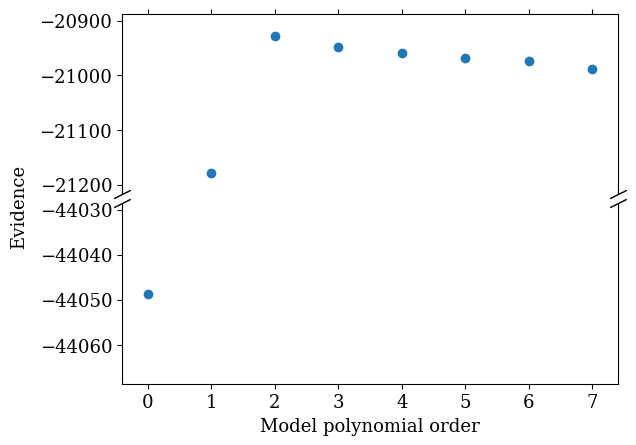
\includegraphics[width=0.5\textwidth]{sim_evidence}
    \caption{Evidence of multiple models are plotted which display the Occam's cliff. Data is generated using noise wave parameters as order-2 polynomials. We see that for the model with the highest evidence, that is, the model favoured by the data, the number of polynomial coefficients matches that of the model noise wave parameters.
    \label{fig:evidence}}
\end{figure}


% =========================================
\subsection{Application with realistic noise}\label{sec:sim_results}
To demonstrate the robustness of our pipeline, we conducted self-consistency checks using empirically modelled data with a more complicated noise model. This data was generated using reflection coefficients of eight calibrators and the receiver measured in the laboratory. These reflection coefficients were then smoothed using a cubic smoothing spline \citep{spline} in order to maintain their approximate shape over frequency. The same second-order noise wave parameters detailed in \cref{sec:opt} are used with the reflection coefficients to generate our model power spectral densities. Following this, we added of order 1\% Gaussian noise independently to the smoothed $\G{rec}$ and $\Ga$ as well as $\psd{cal}$ to more accurately represent the instrument noise from measurement equipment such as vector network analysers. No noise was added to the calibrator input temperatures. This results in a model that does not match the Gaussian form of our mathematical model as in the previous sections and thus does not demonstrate the features of our pipeline as explicitly, but is more representative of data set expected from measurements in the field. Data for the receiver and the cold load generated using this noise model are shown in \cref{fig:calQualities}.
\begin{figure}
    \centering
    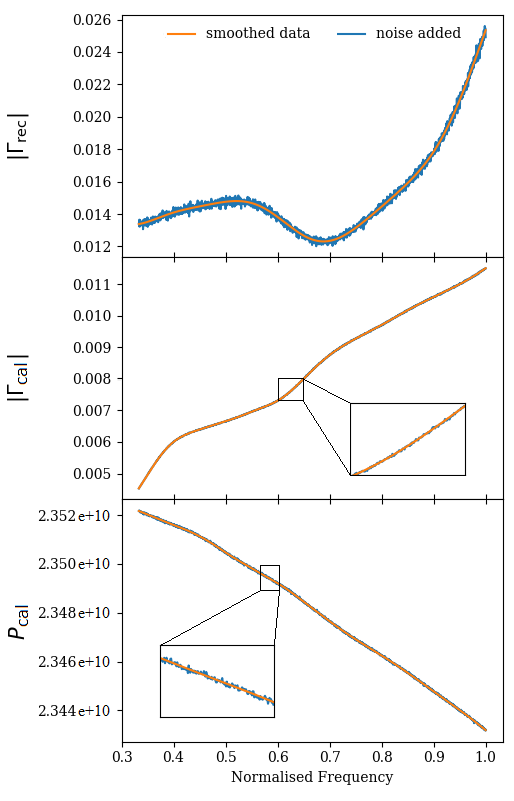
\includegraphics[width=.5\textwidth]{calQualities}
    \caption{Power spectral densities and reflection coefficients for the receiver and the cold load generated under our realistic noise model. 
    \label{fig:calQualities}}
\end{figure}

Using data generated for all eight calibrators with our realistic noise model, the calibration algorithm selects optimal polynomial orders matching those of the model noise wave parameters whose values fall within within $1\sigma$ of the posterior peak values as shown in \cref{fig:fgxSamples}. For these higher order tests, we use fgivenx plots which condense noise wave parameter posteriors into samples that can be compared to the model parameter values instead of comparing each individual coefficient \citep{fgx}.
\begin{figure}
    \centering
    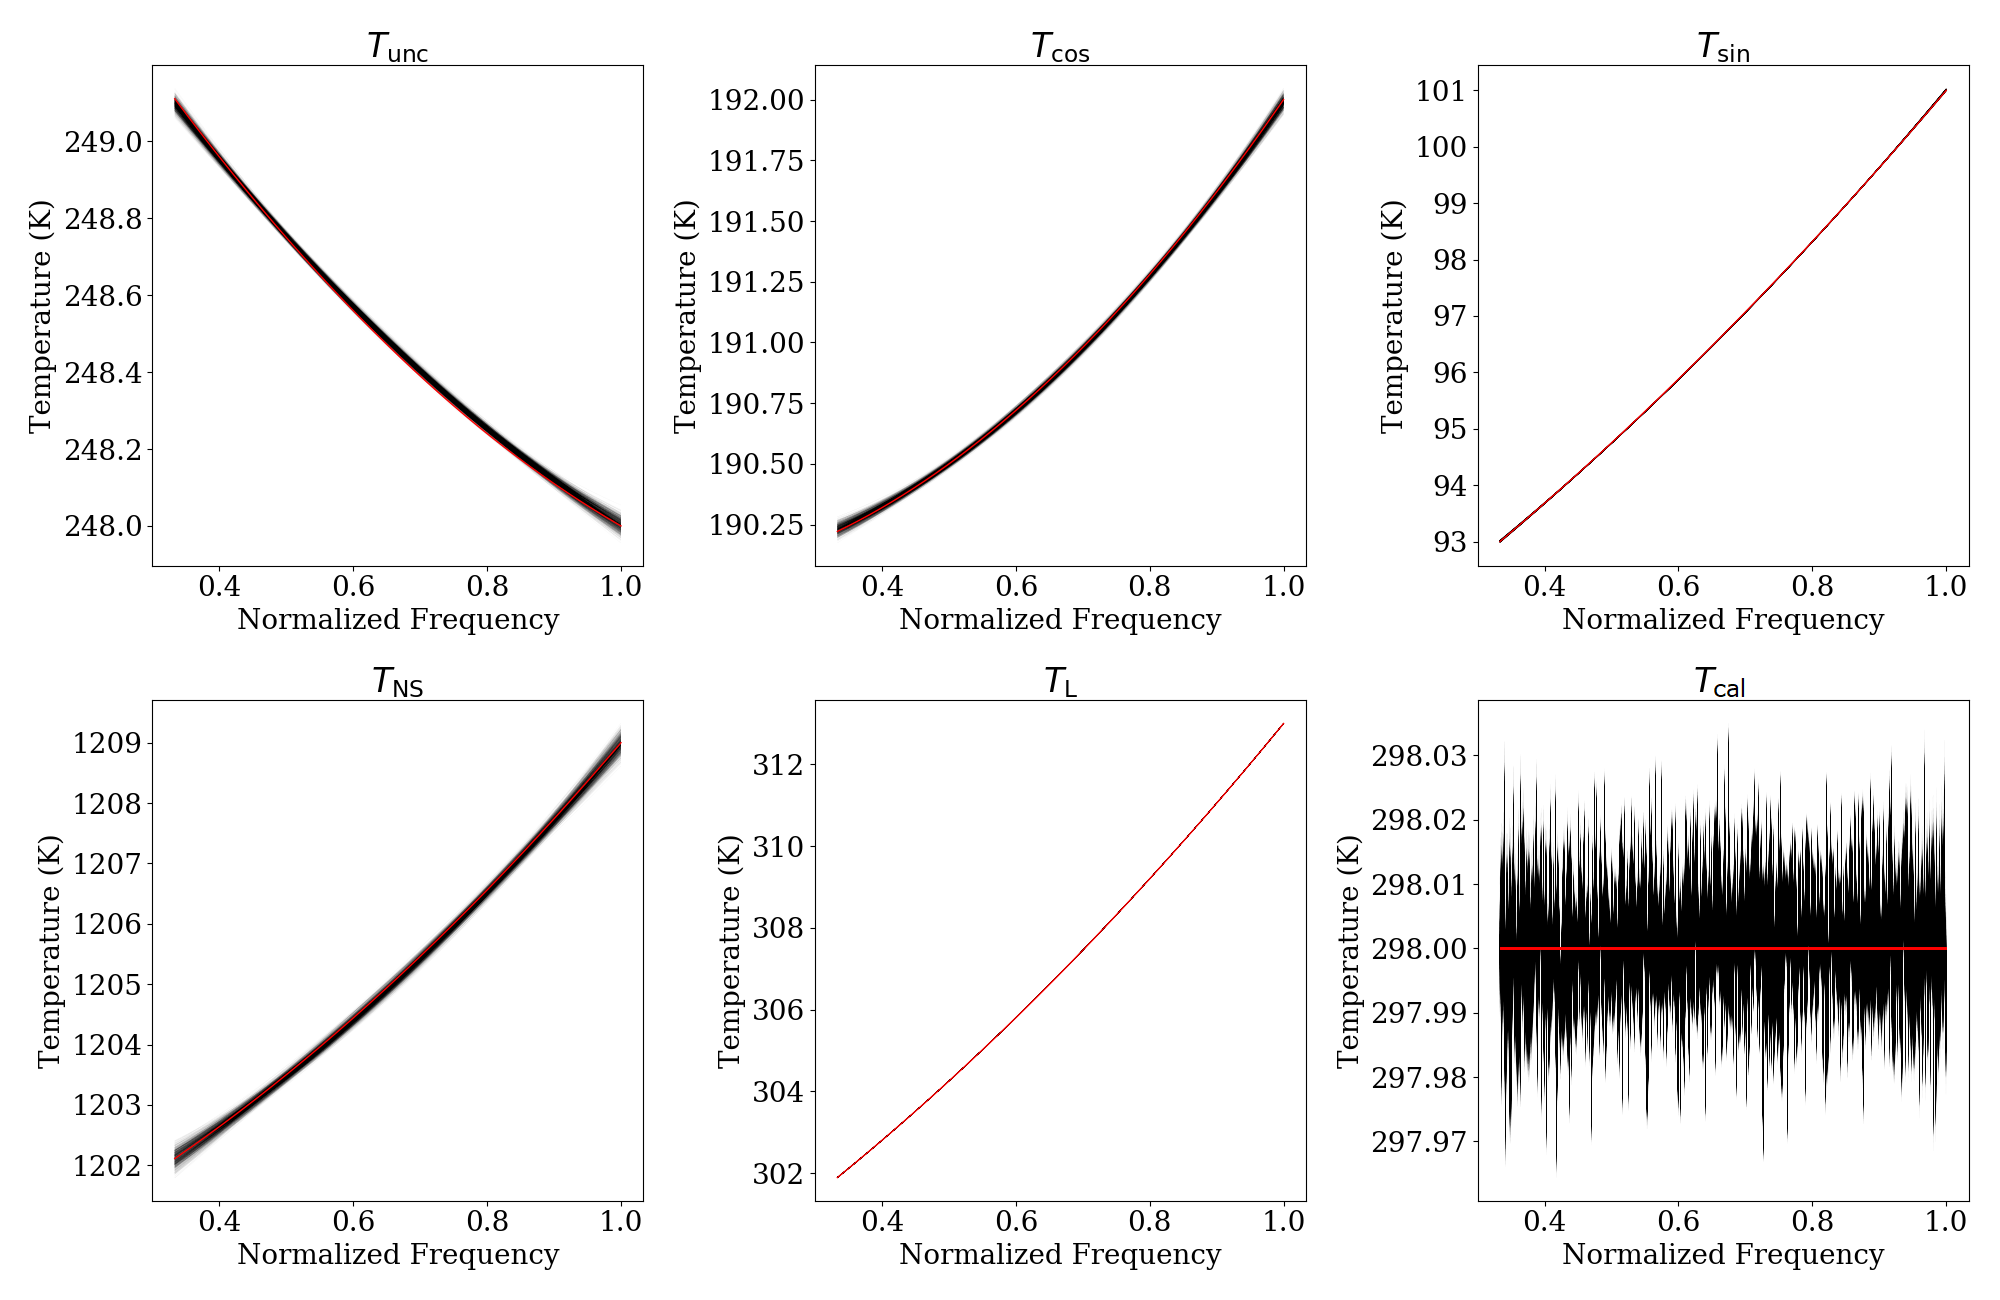
\includegraphics[width=\textwidth]{fgxSamples}
    \caption{Results from 1000 samples using data generated with our more realistic noise model (shown in black). The second-order noise wave parameters shown in red are used to generate the data inputted to our pipeline. The polynomial order and values of the noise wave parameters that best suit the data according to our algorithm match that of the empirical model. This solution is applied to an ambient-temperature load, shown in the bottom right panel as our predictive $\hat{y}$ from \cref{eqn:predictive}, and calibrates it to within $1\sigma$ of ambient temperature. \label{fig:fgxSamples}}
\end{figure}

When this calibration model is used to calibrate an ambient-temperature $50 \ \Omega$ load, the RMS error between the calibrated temperature and the measured temperature is 8 mK, well within the $1\sigma$ noise level (bottom right panel of \cref{fig:fgxSamples}). This level of accuracy is comparable to the 26 mK noise floor estimated for the EDGES pipeline in 2016 \citep{edgesCal}.


% =========================================
\subsection{Waiting for REACH: Results with a HERA receiver}\label{sec:hera_results}
The comparable results of our preliminary technique and the independent EDGES framework serves as a verification of our formulation which would need to be evaluated using real data. While awaiting construction of the REACH hardware a HERA Front End Module (FEM) was employed as a sufficient proxy for data collection. The FEM’s Cambridge-led design and construction, along with HERA’s targeting of similar radio-frequency hydrogen signals ensured that similar technologies were incorporated into its architecture including a switch for comparison of the module input with two internal references. Some of the FEM design considerations accommodating the experimental requirements of HERA needed to be addressed, most notably; a pair of low noise amplifiers between the module input and the internal reference switch. The inclusion of these amplifiers, highlighted in \cref{fig:fem_block}, invalidate the assumption of $g_{\mathrm{sys}} \approx g_{\mathrm{sys}}^*$ for this receiver design. To account for this with minimal changes to our pipeline, we sought to quantify the gain of the FEM’s anterior amplifiers as a corrective factor to be applied to spectral measurements before submission to our pipeline as ordinary data\footnote{This assumes that the gain of the HERA hardware is strictly linear, which is reasonable based on the design specifications.}.
\begin{figure}
    \centering
    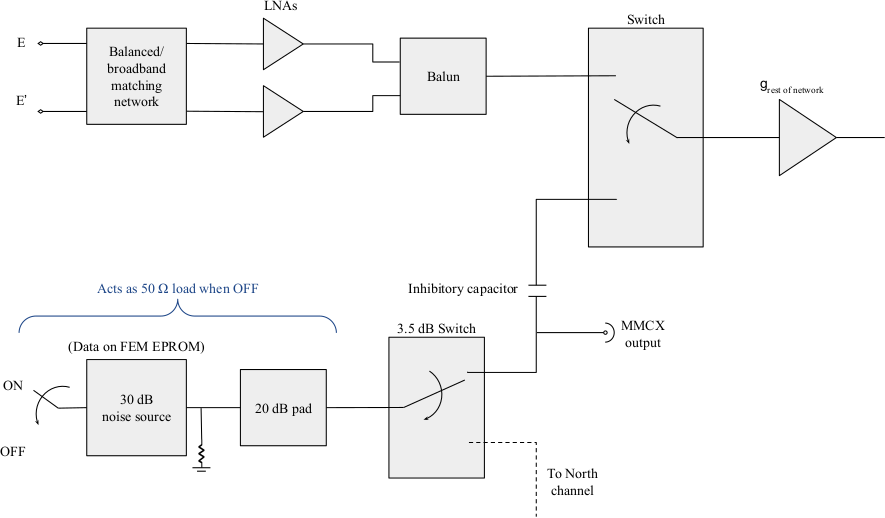
\includegraphics[width=.8\textwidth]{fem_block}
    \caption{A block diagram of the HERA Front End module East channel input. The module input, marked E and E', is immediately followed by two low noise amplifiers before a balun converts the signal to a feed line into the internal switch. The switch toggles between the FEM input and a contraption acting as a passive $50 \Omega$ load or a 6.5 dB noise source when powered. The MMCX output allows for rerouting of the internal reference outputs. The circuitry following the internal switch approximates that of the REACH front-end receiver, permitting normal operation of our calibration procedure.}
    \label{fig:fem_block}
\end{figure}

Appraisal of the FEM amplifiers required physical modifications to the device such as the removal of an inhibitory capacitor to impedance match the internal references with the rest of the circuit. Following this, the internal switch measures the references directly without amplification. An MMCX output linked to the internal references is then used to redirect their output to the module input where the data would pass through the low noise amplifiers before being measured. An image of the setup used to reroute the internal references to the FEM input is shown in \cref{fig:hera_reroute}.
\begin{figure}
    \centering
    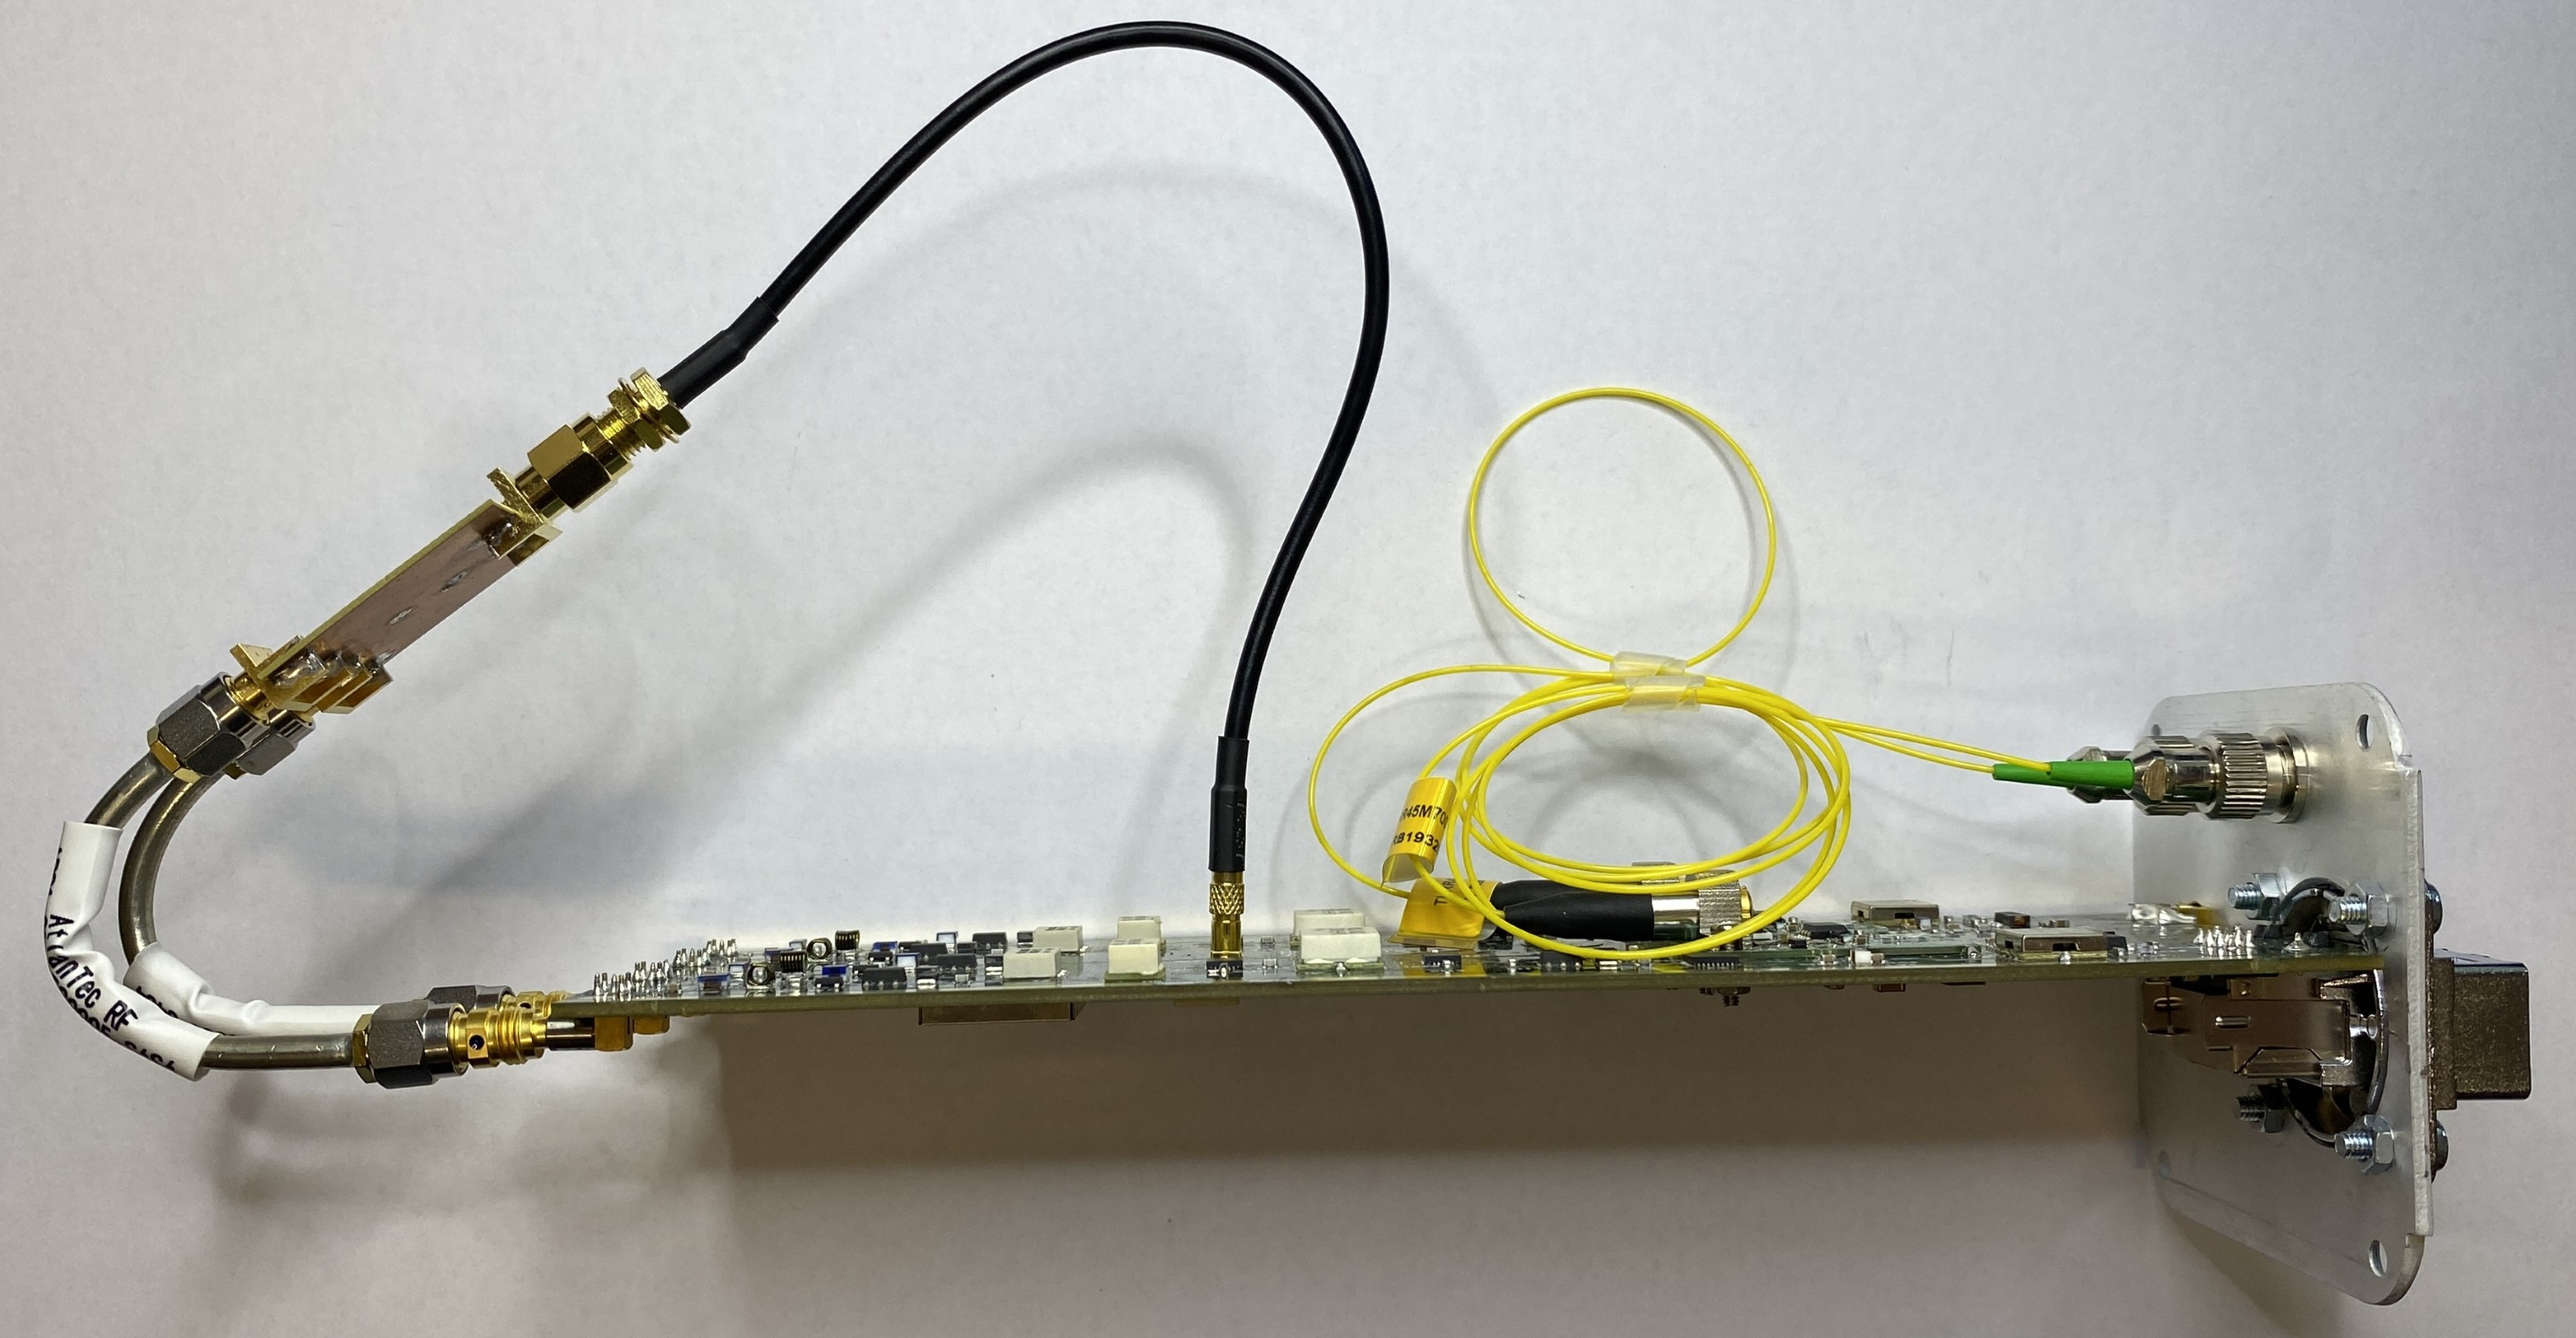
\includegraphics[width=.8\textwidth]{hera_reroute}
    \caption{A HERA Front End Module without its housing, configured to evaluate anterior LNA gain. At the board's centre is the internal reference MMCX output connected to a hybrid splitter which bisects the signal into a pair separated by a $180^{\circ}$ phase difference. The signal is then directed to the module input for measurement of the amplifier effects on the internal references.}
    \label{fig:hera_reroute}
\end{figure}
As shown in \cref{fig:mmcx_compare}, the amplified reference load signal resembles an upward shift and broadening of the direct signal, which we approximate as a frequency-dependent multiplicative factor executed by the LNAs. The same behaviour can be seen in the internal noise source data (not shown) and is consistent over multiple data runs. We therefore compile spectral data for this receiver in a three-step process; 1) measurement of the calibrators at the module input followed by 2) direct measurement of the Dicke references via internal switch. 3) The corrective factors derived from the MMCX output procedure are then applied to the internal reference load and noise source data to effectively equalise the gain over all spectral data before being passed to our pipeline as an ordinary dataset. This operation allowed us to avoid the complications of manually switching the calibration sources and rerouted reference signals at the FEM input when ‘cycling’ through the Dicke switch.
\begin{figure}
    \centering
    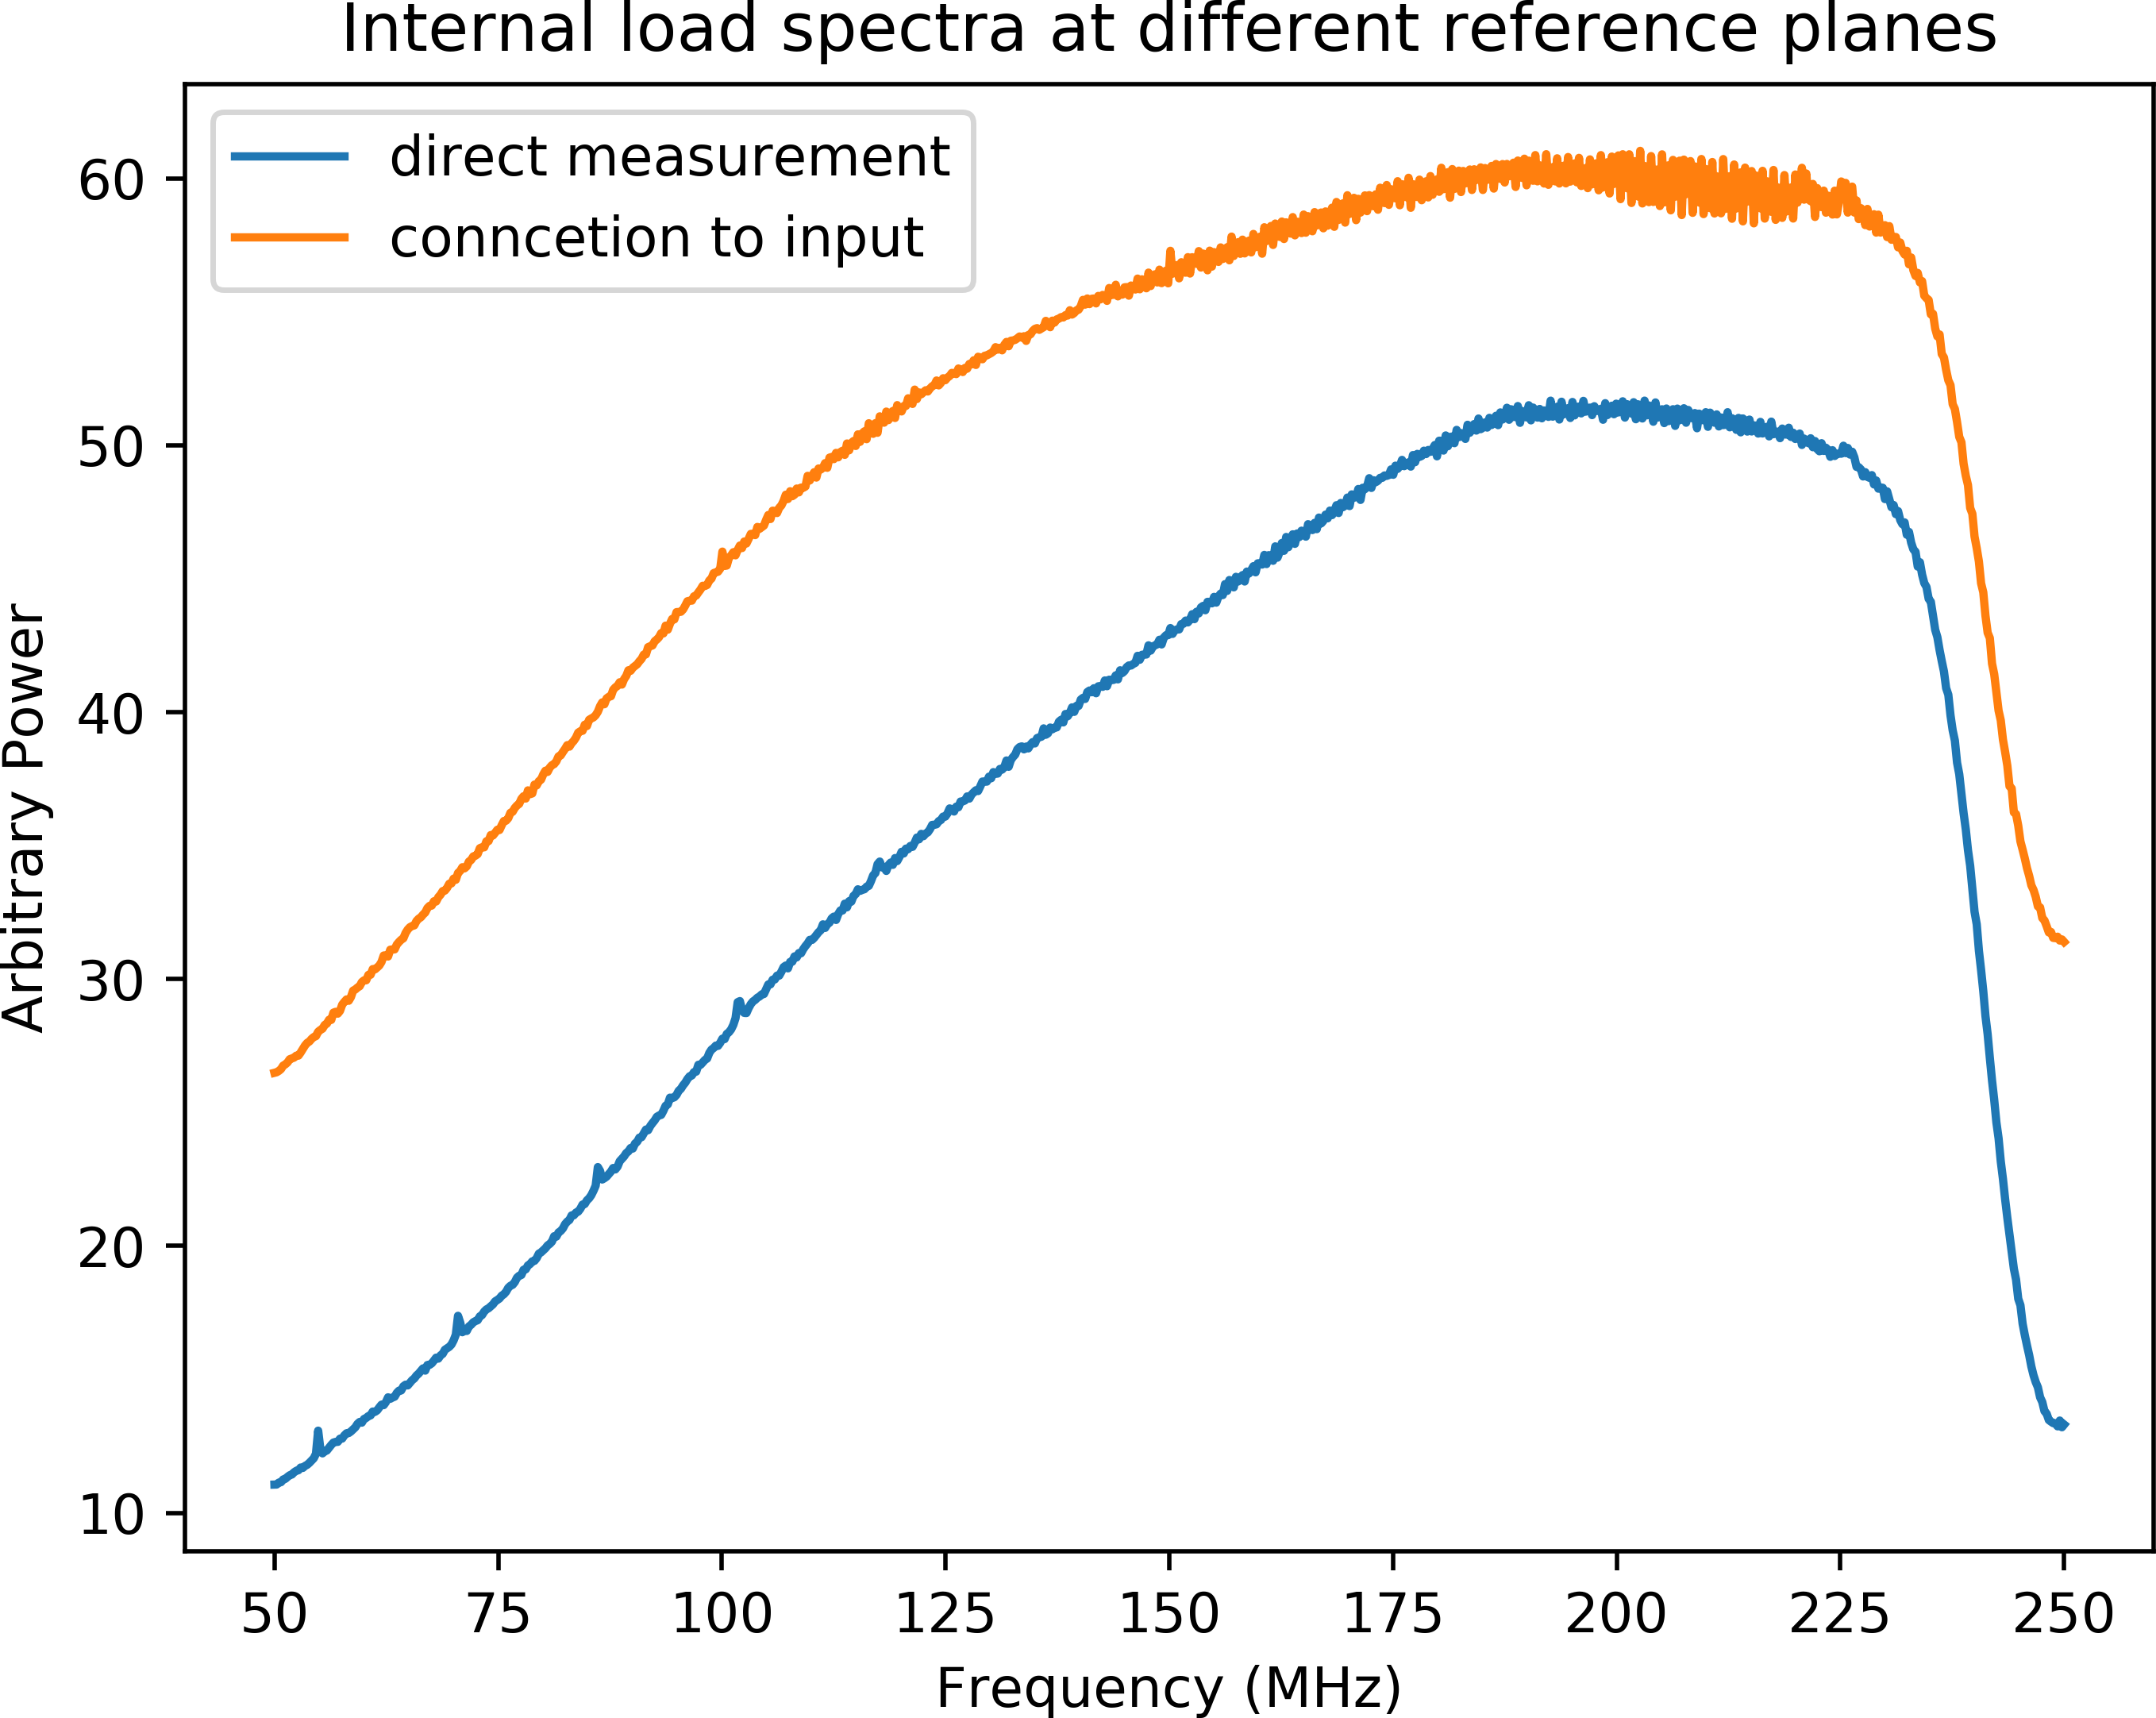
\includegraphics[width=.6\textwidth]{mmcx_compare}
    \caption{Comparison of data from the reference load when measured directly thorough the internal switch (blue) and when directed to the module input via MMCX output (orange). The apparent action of the amplifiers on the redirected data can be approximated as a frequency-dependent multiplicative factor which is applied to the internal reference data before submission to our pipeline.}
    \label{fig:mmcx_compare}
\end{figure}

As the internal reference connection to the module input shown in \cref{fig:hera_reroute} prevented use of the FEM in its regular housing, data collection was undertaken with the device placed in a RF-secure chamber similar to the Rittal AE 1007.600 enclosure detailed in \cref{sec:frontend}. The FEM output was connected to the same iTPM used for REACH acting as a spectrometer and reflection data was taken with a Keysight N5247A PNA-X. A single temperature reading was recorded at the beginning of each device's respective spectral measurement via thermocouple.

Under this configuration, four calibrators were used; an ambient temperature $50 \Omega$ load, a $50 \Omega$ load heated to 373 K, a 12.5 metre TCOM-200 cable with an opened end, and the same cable with a shorted end. The derived solution was then calibrated against an ambient temperature HERA noise filter. The results, plotted in \cref{fig:hera_results}, show 1000 model samples from our posterior achieving a 236 mK RMS error and a noise term $\sigma = 3.942$ K under our formulation THERE SHOULD BE AN EQUATION FOR SIGMA SOMEWHERE. While the sub-kelvin error is encouraging, the solution however does not centre on the temperature of the noise filter measured to be 300.4 K. It is understood that more accurate measurements of the $50 \Omega$ load calibration sources would improve this as adjustments to this data translate the solution up and down accordingly. This finding informed the design of the REACH front-end to record temperature over the entire period of a calibrator’s spectral measurement. Also seen in the solution is sinusoidal structure across the entire bandwidth suggesting a systematic not being accounted for. As the load-based calibrators determine the temperature scale of the solution, the cable-based sources characterise its shape, e.g. cable information is somehow not being captured by our algorithm. Repeated results such as these were the motivation to include a more accurate temperature model for the cable calibration sources as detailed in REFERENCE SECTION ON CABLE CORRECTION. We also note that the calibration accuracy using a HERA FEM is limited by the Noisecom NC4959 used as the reference noise source, which varies in output by $\sim1$ dB compared to the NC346A used in the REACH front-end which varies by 0.2 dB over the observation band (see \cref{tab:ns_noise}). We therefore believe that our RMSE of $\sim200$ mK approaches the limit for this particular device using our algorithm. A full schematic of the HERA FEM as well as images of the circuit board are given in \cref{fig:fem_schematic} and \cref{fig:fem} for reference.
\begin{figure}
    \centering
    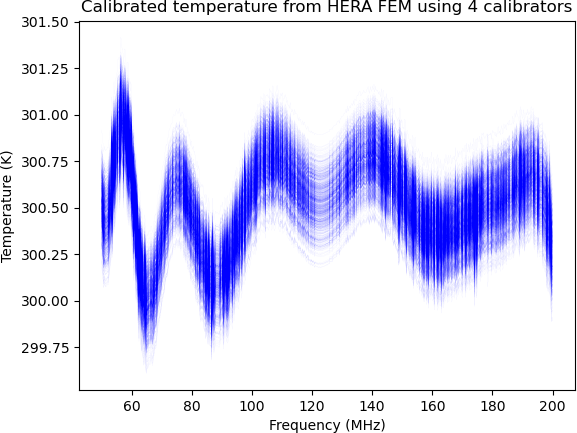
\includegraphics[width=.8\textwidth]{hera_results}
    \caption{1000 posterior samples from our calibration algorithm using data collected with a HERA FEM are shown in blue. The solution is derived from four canonical sources calibrated against an ambient-temperature noise filter. The integration time for spectral measurements was not recorded for this experiment but was likely 2 minutes as this was our standard for such experiments. While the solutions exhibit a 236 mK RMS error, they do not centre on the measured temperature of the noise filter at 300.4 K shown in red. Ignoring the measured noise filter temperature, the RMSE of the 1000 samples from their average shown in yellow is 212 mK. Sinusoidal structure can be seen across the bandwidth suggesting a cable-based systematic not being captured by our technique.}
    \label{fig:hera_results}
\end{figure}


% =========================================
\subsection{REACH Results?}\label{sec:reach_results}
Data collection using the REACH receiver system commenced once the majority of construction was completed. In the laboratory, automated data sets were taken using the front and back-ends linked by 100 metres of fibre cabling wound over a spool to represent the entire length of the signal chain deployed in South Africa (\cref{fig:fibre_spool}).
\begin{figure}
    \centering
    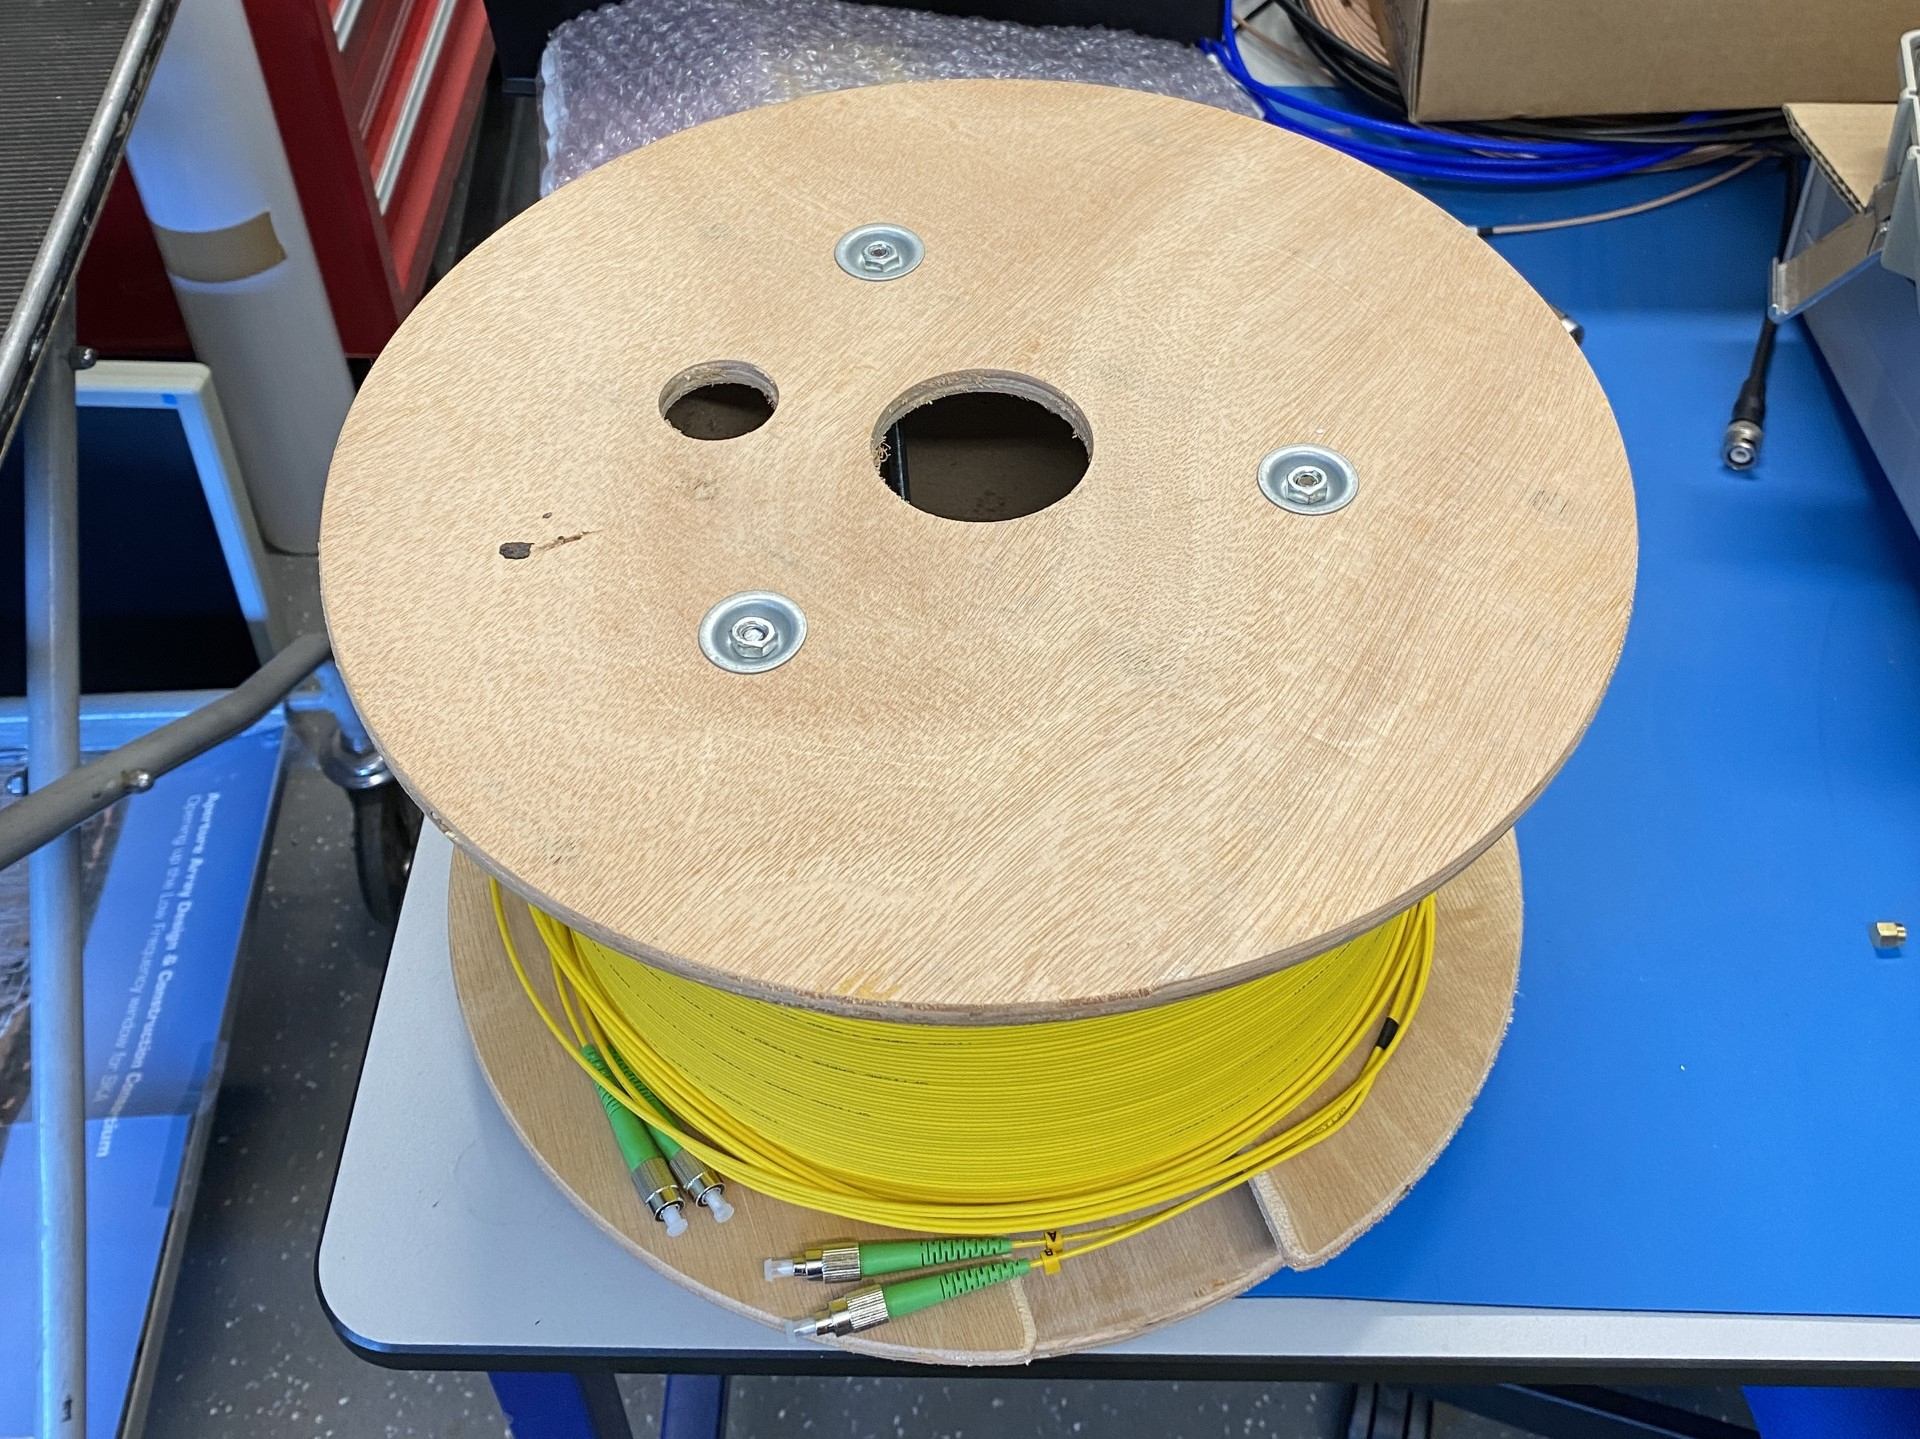
\includegraphics[width=.6\textwidth]{fibre_spool.jpg}
    \caption{Due to space constraints within the lab, 100 metres of fibre optic cabling were wound over a spool to verify communication between the receiver front and back-end units over the planned deployment separation as detailed in \cref{sec:receiver_general}.}
    \label{fig:fibre_spool}
\end{figure}

\subsubsection{Mock antenna results 1}
An initial dataset was taken using all 12 calibration sources detailed in \cref{sec:frontend} integrated for two minutes each (e.g two minute integrations on the source, then two minutes on the reference load, followed by two minutes on the reference noise source, repeated for each calibration source). For this particular experiment, it should be noted that data was taken with the front-end components assembled outside of the thermal enclosure, which is expected to negatively affect calibration accuracy. The resulting calibration solution is applied to an ambient-temperature noise filter used as our mock antenna as in the previous section. A plot of 1000 sampled solutions, shown in \cref{fig:reach_results_1}, once again does not centre on the measured mock antenna temperature of 302.8 K and achieves an RMSE of 1.075 with respect to it. An RMSE recalculated with respect to the sample average is 689 mK and our posterior error term $\sigma=4.041$ K.
\begin{figure}
    \centering
    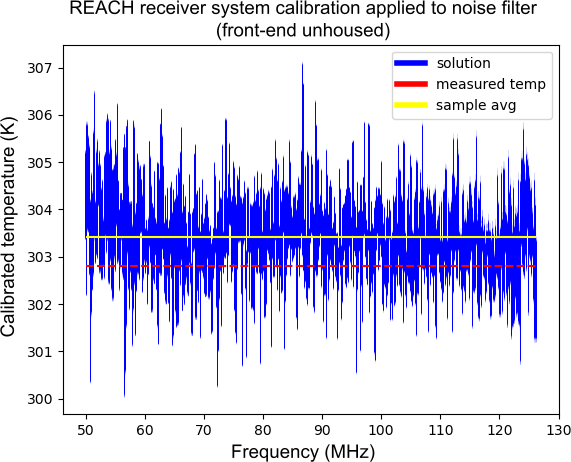
\includegraphics[width=.8\textwidth]{reach_results_1}
    \caption{1000 posterior samples from our calibration pipeline using data taken with the REACH receiver system is shown in blue. The front-end did not have its enclosure during data collection for this experiment. All twelve calibration sources were integrated for two minutes and the solution was applied to a room temperature noise filter as our mock antenna. The measured antenna temperature is 302.8 K (red line) which differs from the sample average (yellow), however less structure can be seen than in \cref{fig:hera_results}. The RMSE is 1.075 K with respect to the measured antenna temperature and 689 mK with respect to the sample average. Our posterior error term $\sigma=4.041$ K.}
    \label{fig:reach_results_1}
\end{figure}

These results using the REACH receiver system exhibit much less structure than that of the HERA FEM, however the solution still does not resemble Gaussian noise as would be expected from a successful calibration. The average of the posterior samples shown in yellow once again does not correspond to the measured temperature of the mock antenna shown in red. There are also a few spikes in the solution that stand out qualitatively which we take to be RFI. We attribute the defects of our results to the absence of the front-end enclosure and the lack of its accompanying features such as the thermal management subsystem and RFI shielding. We also note the differences between the reported root mean square errors and our error term, $\sigma$. We approached this by reformulating our priors starting with setting the prior on our shape parameter
\begin{equation}
    a = 1,
    \label{eqn:alpha_reform}
\end{equation}
which, for our inverse-gamma prior, corresponds to being very wide while still remaining normalised. We see in MEAN VARIANCE EQUATIONS IN INV-GAM DISTRIBITION WIKIPEDIA PAGE, that there is no mean or variance for $a=1$, indicating that the distribution is heavily tailed while reaching a peak at $b/(a + 1)$. Our prior for the scale parameter is therefore 
\begin{equation}
    b = \left(a + 1\right) \times \left(\frac{\sigma_{p}}{300}\right)^2.
    \label{eqn:beta_reform}
\end{equation}
Here $\sigma_{p}$ is the level of noise which we expect to find which we appraise to be $\sim 1$ K based on our instrument construction. Additionally, $b$ is normalised by our assumed ambient temperature of 300 K which is then squared, giving $b$ dimensions of temperature squared. Our priors for the statistical spread of each of our five noise wave parameter values are set to 10. Given the $a + 1$ term in \cref{eqn:beta_reform}, this corresponds to five $\sigma$ widths and is dimensionless. We can confirm that the results are relatively insensitive to changes in the priors for our noise wave parameter values as the priors are very wide and we use a large amount of training data. Using our formulation for our updated prior volume $\mathbfss{V}^*$ in \cref{starred}, our posterior error term
\begin{equation}
    \sigma^2 = \Sigma^* = \left( \frac{b^*}{a^*} \right) \mathbfss{V}^*,
    \label{eqn:sigma_reform}
\end{equation}
which has dimensions of normalised temperature. We believe this reformulation to be robust and verified that the expected results are recovered using simulated data.

\subsubsection{Mock antenna results 2}
As we continued to construct the receiver, many components required replacement including the TEC power supply, VNA, iTPM and the USB-to-fibre converter. While we do not expect these replacements to affect our calibration results, we report them here for the sake of documentation or consideration in future analyses. To better assess the capabilities of our pipeline, a mock antenna was built to resemble the $S_{11}$ of the deployed antenna dipole based on simulations provided by CITE JOHN CUMNER. This mock antenna was made by soldering a $90 \Omega$ load to the end of a 2 metre coaxial cable, providing an $S_{11}$ varying between -11 dB and -14 dB as shown in \cref{fig:s11_meas}. With this configuration, 16-minute integrations were performed on eight calibration sources; the ambient and heated $50 \Omega$ loads, shorted and open cables, $25 \Omega$ and $100 \Omega$ resistors, and the 12 metre calibration cable terminated at $27 \Omega$ and $91 \Omega$. The calibration solution applied to our mock antenna is shown in \cref{fig:reach_results_2} and yields a $\sigma = 1.464$ K.
\begin{figure}
    \centering
    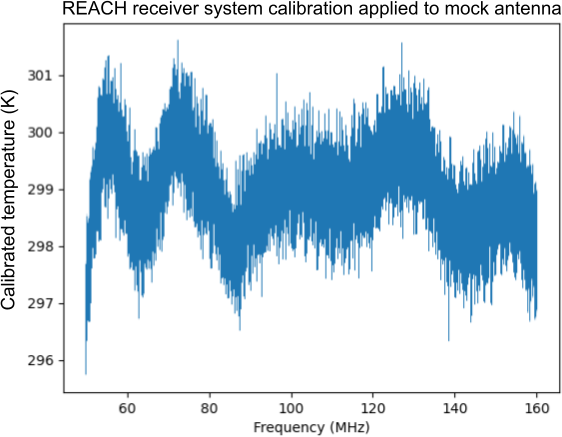
\includegraphics[width=0.8\textwidth]{reach_results_2}
    \caption{1000 posterior samples from our calibration pipeline using data taken with the completed REACH receiver system including the front-end enclosure. Eight calibration sources were integrated for 16 minutes and the resulting solution was applied to a new mock antenna resembling the reflection characteristics of the deployed antenna dipole. A posterior error $\sigma = 1.464$ K is achieved.}
    \label{fig:reach_results_2}
\end{figure}
The calibration results are seen to have a clear sinusoidal systematic which we attribute to some physical phenomena not being accounted for or incorporated into our pipeline.

\section{Responses}
The sinusoidal structure seen in both \cref{fig:hera_results} and \cref{fig:reach_results_2} indicate systematics needing to be addressed. The two typical avenues of approach are to; a) find and attend to the physical source of the systematic (loose wire, etc) and b) incorporate better numerical models into our algorithm to incorporate the information not captured presently. For the engineer, the former is often attempted first, and for the statistician, the latter. One may argue that a perfect calibration algorithm should account for any systematic, which perhaps is true. In practice however, incorporating a myriad of models for every potential loose wire at every connection or the impedance changes of every component with every degree of temperature increase proves difficult. The approach of identifying physical faults with the instrument tends to yield more immediate results as well, as shown in \cref{fig:lna_switched_reach_result} where the front-end low noise amplifier was replaced with a new construction of identical specifications.
\begin{figure}
    \centering
    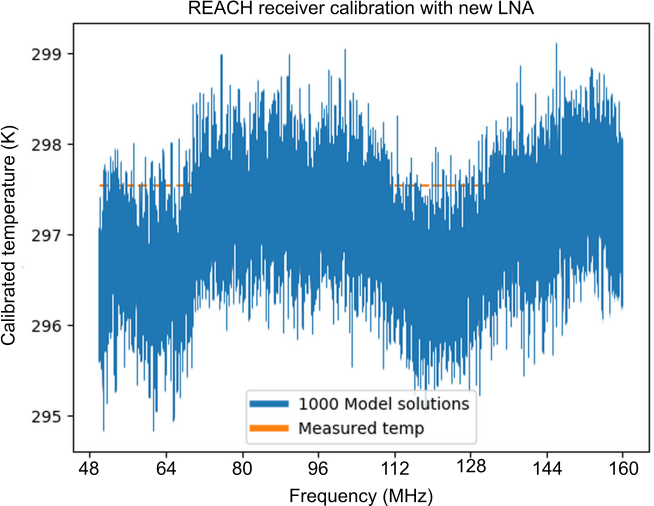
\includegraphics[width=0.8\textwidth]{lna_switched_reach_result}
    \caption{Results from our calibration pipeline using data taken as in \cref{fig:reach_results_2} but with a new LNA built to identical specifications. As can be seen, some of the sinusoidal structure has been ameliorated suggesting that a component within the original LNA was partially at fault. 1000 posterior samples are shown in blue. Eight calibration sources were integrated for 16 minutes and the resulting solution was applied to the mock antenna. The posterior error is $\sigma = 1.070$ K.}
    \label{fig:lna_switched_reach_result}
\end{figure}

The results of \cref{fig:lna_switched_reach_result} show a marked decrease in sinusoidal structure, but still exhibits systematics indicating the need for further adjustment. A great deal of attempts to physically rectify the systematic were made that provided little or no improvements to the results. We first recollected datasets with increased and decreased out-of-band 10 MHz tone injection through the application or removal of attenuators at the amplifier output. This was thought to better calibrate short-term variation in the spectrometer over the course of the three-position Dicke cycle during measurements through the division of power spectral measurements in \cref{eqn:tantstar}, though no change in results were seen. We next took datasets at different front-end TEC setpoints, having it maintain a variety of different temperatures. While the calibration results did not improve for these runs, we can confirm that instructing the machine to maintain a set point closer to the outside ambient temperature has beneficial effects on the power consumption of the machine, as one would expect.

Following this, we noted the possibility of a small, hertz or kilohertz-level misalignment of measurement frequency bins between the VNA and spectrometer due to the devices being separate machines taking independent frequency measurements. In response to this, we employed a Stanford Research Systems FS725 Rubidium Frequency Standard as an external reference connected to the VNA and spectrometer for a true frequency-by-frequency bin matchup. While data sets using this setup did not yield noticeable improvement, suggesting that at the current calibration scale, kilohertz or lower level bin misalignment would not affect our measurements, we recommend the alignment of the VNA and spectrometer through a similar configuration for future builds. In principle, this would be beneficial as calibration accuracy improves past the ten millikelvin level.

We then proceeded to replace every individual component within the receiver including every switch, the VNA, iTPM spectrometer and USB-to-fibre converters. We experimented with both longer and shorter calibration cables as well as different brands of cabling. The calibration sources were rebuilt and a battery of attenuators and ferrite beads were installed throughout the instrument to reduce any internal electromagnetic interference. Filtering of the RF signals was also tried with no effect. Adjustments were made to the VNA sweep time to compensate for any delays in the signal travelling up and down the length of the calibration cables. We even attempted data runs in which spectral data was taken as normal while reflection data was taken by the Keysight N5247A PNA-X to determine whether or not the specifications of the CMT TR1300/1 were the limiting factor, which was not found to be the case. Setups with the PNA-X and spectrometer aligned by the FS725 Rubidium standard were also investigated with still no rectification of the systematics seen in the results.

We consider the above to be the extent of reasonable adjustments to the physical machine and continue on to the statistician’s approach to systematics--adjustments to our numerical algorithm. We started with reformulating of our priors similar to the procedure of \cref{eqn:alpha_reform} through \cref{eqn:sigma_reform} under various assumptions such as keeping the priors wide or constraining them based off of noise wave parameter values published by EDGES as well as from our own experience. We however considered equations presented in this chapter to be a good compromise between the best calibration accuracy and the wide priors expected of a comparable frequentist approach. We also experimented with the incorporation of additional corrective factors to compensate unaccounted gain contributions as well as offset factors to correct for minute differences in the measurement reference planes. We improved the gradient descent algorithm that optimises the noise wave parameter polynomial order by refactoring the code to avoid getting trapped at local minima. Furthermore, we tried smoothing of the data as well as up-sampling and down-sampling of the data.

\section{Additional models for incorporation}
In our experimentation with modifications of our algorithm, we decided on three additional models to be incorporated into our calibration procedure. While these models do not result in immediate practical benefits to our experimental results with regard to the sinusoidal systematics presented above, they serve to reinforce the theoretical foundation on which our algorithm is built. These models are explained below.

\subsection{Fixture compensation to improve S-parameter measurements}\label{sec:tparameters}
At our desired levels of precision, RF system design must minimise the number of reference planes within the instrument. Each additional reference plane will have its own path-specific signal delays and reflections which slightly alter the data with respect to a measurement device such as the VNA. Preceding the full calibration of the receiver, the VNA is initially calibrated via the SOL standards with respect to the MS2 input reference plane as shown in \cref{fig:overview}. Following this, all further reflection measurements of the calibration sources and LNA are taken with respect to a reference plane at the inputs of the MTS switch, represented by the red dashed lines in \cref{fig:overview}\footnote{We take the mechanical switches MS1, MS3 and MS4 to be lossless while assuming the path through the 2-port MTS is non-negligible.}.

Omitting any redesign of the front-end, we may attempt to mitigate the effects of the path length through the MTS switch through the techniques of fixture compensation. A particularly accurate method of fixture compensation is the use of scattering transfer parameters (T-parameters), also referred to as ABCD parameters\footnote{An alternative convention known as chain scattering parameters are also referred to as ‘T-parameters’ and care should be taken to ensure that one’s calculations are consistent to avoid errors} \citep{pozar}. Modelling the MTS+source combination as a cascaded network at the MS2 input reference plane, we may use T-parameters to mathematically de-embed fixtures such as the MTS and remove their effects on the data. For a 2-port network such as the path through the MTS switch, the relation between S-parameters and T-parameters under the scattering transfer convention is defined as
\begin{equation}
    T = \begin{bmatrix}
        T_{11} & T_{12} \\
        T_{21} & T_{22}
    \end{bmatrix}
    =
    \begin{bmatrix}
        \frac{S_{12}S_{21}-S_{11}S_{22}}{S_{21}} & \frac{S_{11}}{S_{21}} \\
        \frac{-S_{22}}{S_{21}} & \frac{1}{S_{21}}
    \end{bmatrix},
    \label{eqn:tparams}
\end{equation}
where the S-parameters in the above matrix are reflection measurements of the offending paths through the MTS switch (e.g. the MTS-J1$\rightarrow$MTS-J2 path for calibration sources and MTS-J3$\rightarrow$MTS-J4 for the LNA). In the current analysis, measurements of the MTS switch were performed in the laboratory using the Keysight N5247A PNA-X. While this procedure contradicts our philosophy of an all-in-field calibration system, we believe it strengthens the foundation of our overall technique and future work will  be undertaken on a system design that either avoids multiple reference planes or facilitates in situ 2-port measurements of the MTS switch.

During a reflection measurement, all the VNA sees is a device under test (DUT) which in reality consists of a calibration source connected to the MTS as shown in \cref{fig:cascaded_network_diagram}. 
\begin{figure}
    \centering
    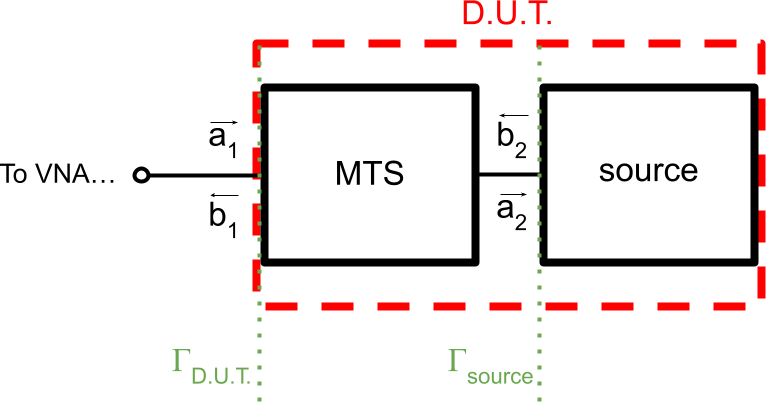
\includegraphics[width=.9\textwidth]{cascaded_network_diagram}
    \caption{From the perspective of the VNA, a reflection measurement is taken of a single device under test (D.U.T.) consisting of the MTS switch connected to a source. The reflection coefficient measured by the VNA, $\G{\mathrm{D.U.T.}}$, is altered by the path through the MTS switch. The desired reading is $\G{\mathrm{source}}$ which needs to be extracted from the D.U.T. measurement.}
    \label{fig:cascaded_network_diagram}
\end{figure}
The traversing and reflected waves are related by
\begin{equation}
    \begin{bmatrix}
        a_1 \\ b_1
    \end{bmatrix}
    =
    \begin{bmatrix}
        T_{11} & T{12} \\
        T_{21} & T{22}
    \end{bmatrix}
    \begin{bmatrix}
        a_2 \\ b_2
    \end{bmatrix},
\end{equation}
where $\G{\mathrm{source}} = \frac{b_2}{a_2}$ and $\G{\mathrm{D.U.T.}} = \frac{b_1}{a_1}$. Wanting the reflection coefficient of the source, we expand as a system of equations that can be solved yielding
\begin{equation}
    \G{source} = \frac{ \G{\mathrm{D.U.T.}} - S_{22}^{\mathrm{MTS}} }{ S_{12}^{\mathrm{MTS}} S_{21}^{\mathrm{MTS}} + S_{11}^{\mathrm{MTS}} \left( \G{\mathrm{D.U.T.}} - S_{22}^{\mathrm{MTS}} \right) },
\end{equation}
where the S-parameters are measurements of the MTS-J1$\rightarrow$MTS-J2 paths for corrections regarding sources and MTS-J3$\rightarrow$MTS-J4 for corrections of the LNA reflection coefficient. These corrections are applied to all S-parameter measureents.

Using simulations of a similar cascaded network made with Keysight’s PathWave RF Synthesis software, we can confirm that this method of fixture compensation retrieves the source reflection coefficient to within six decimal places as shown in \cref{fig:tparam}.
\begin{figure}
    \centering
    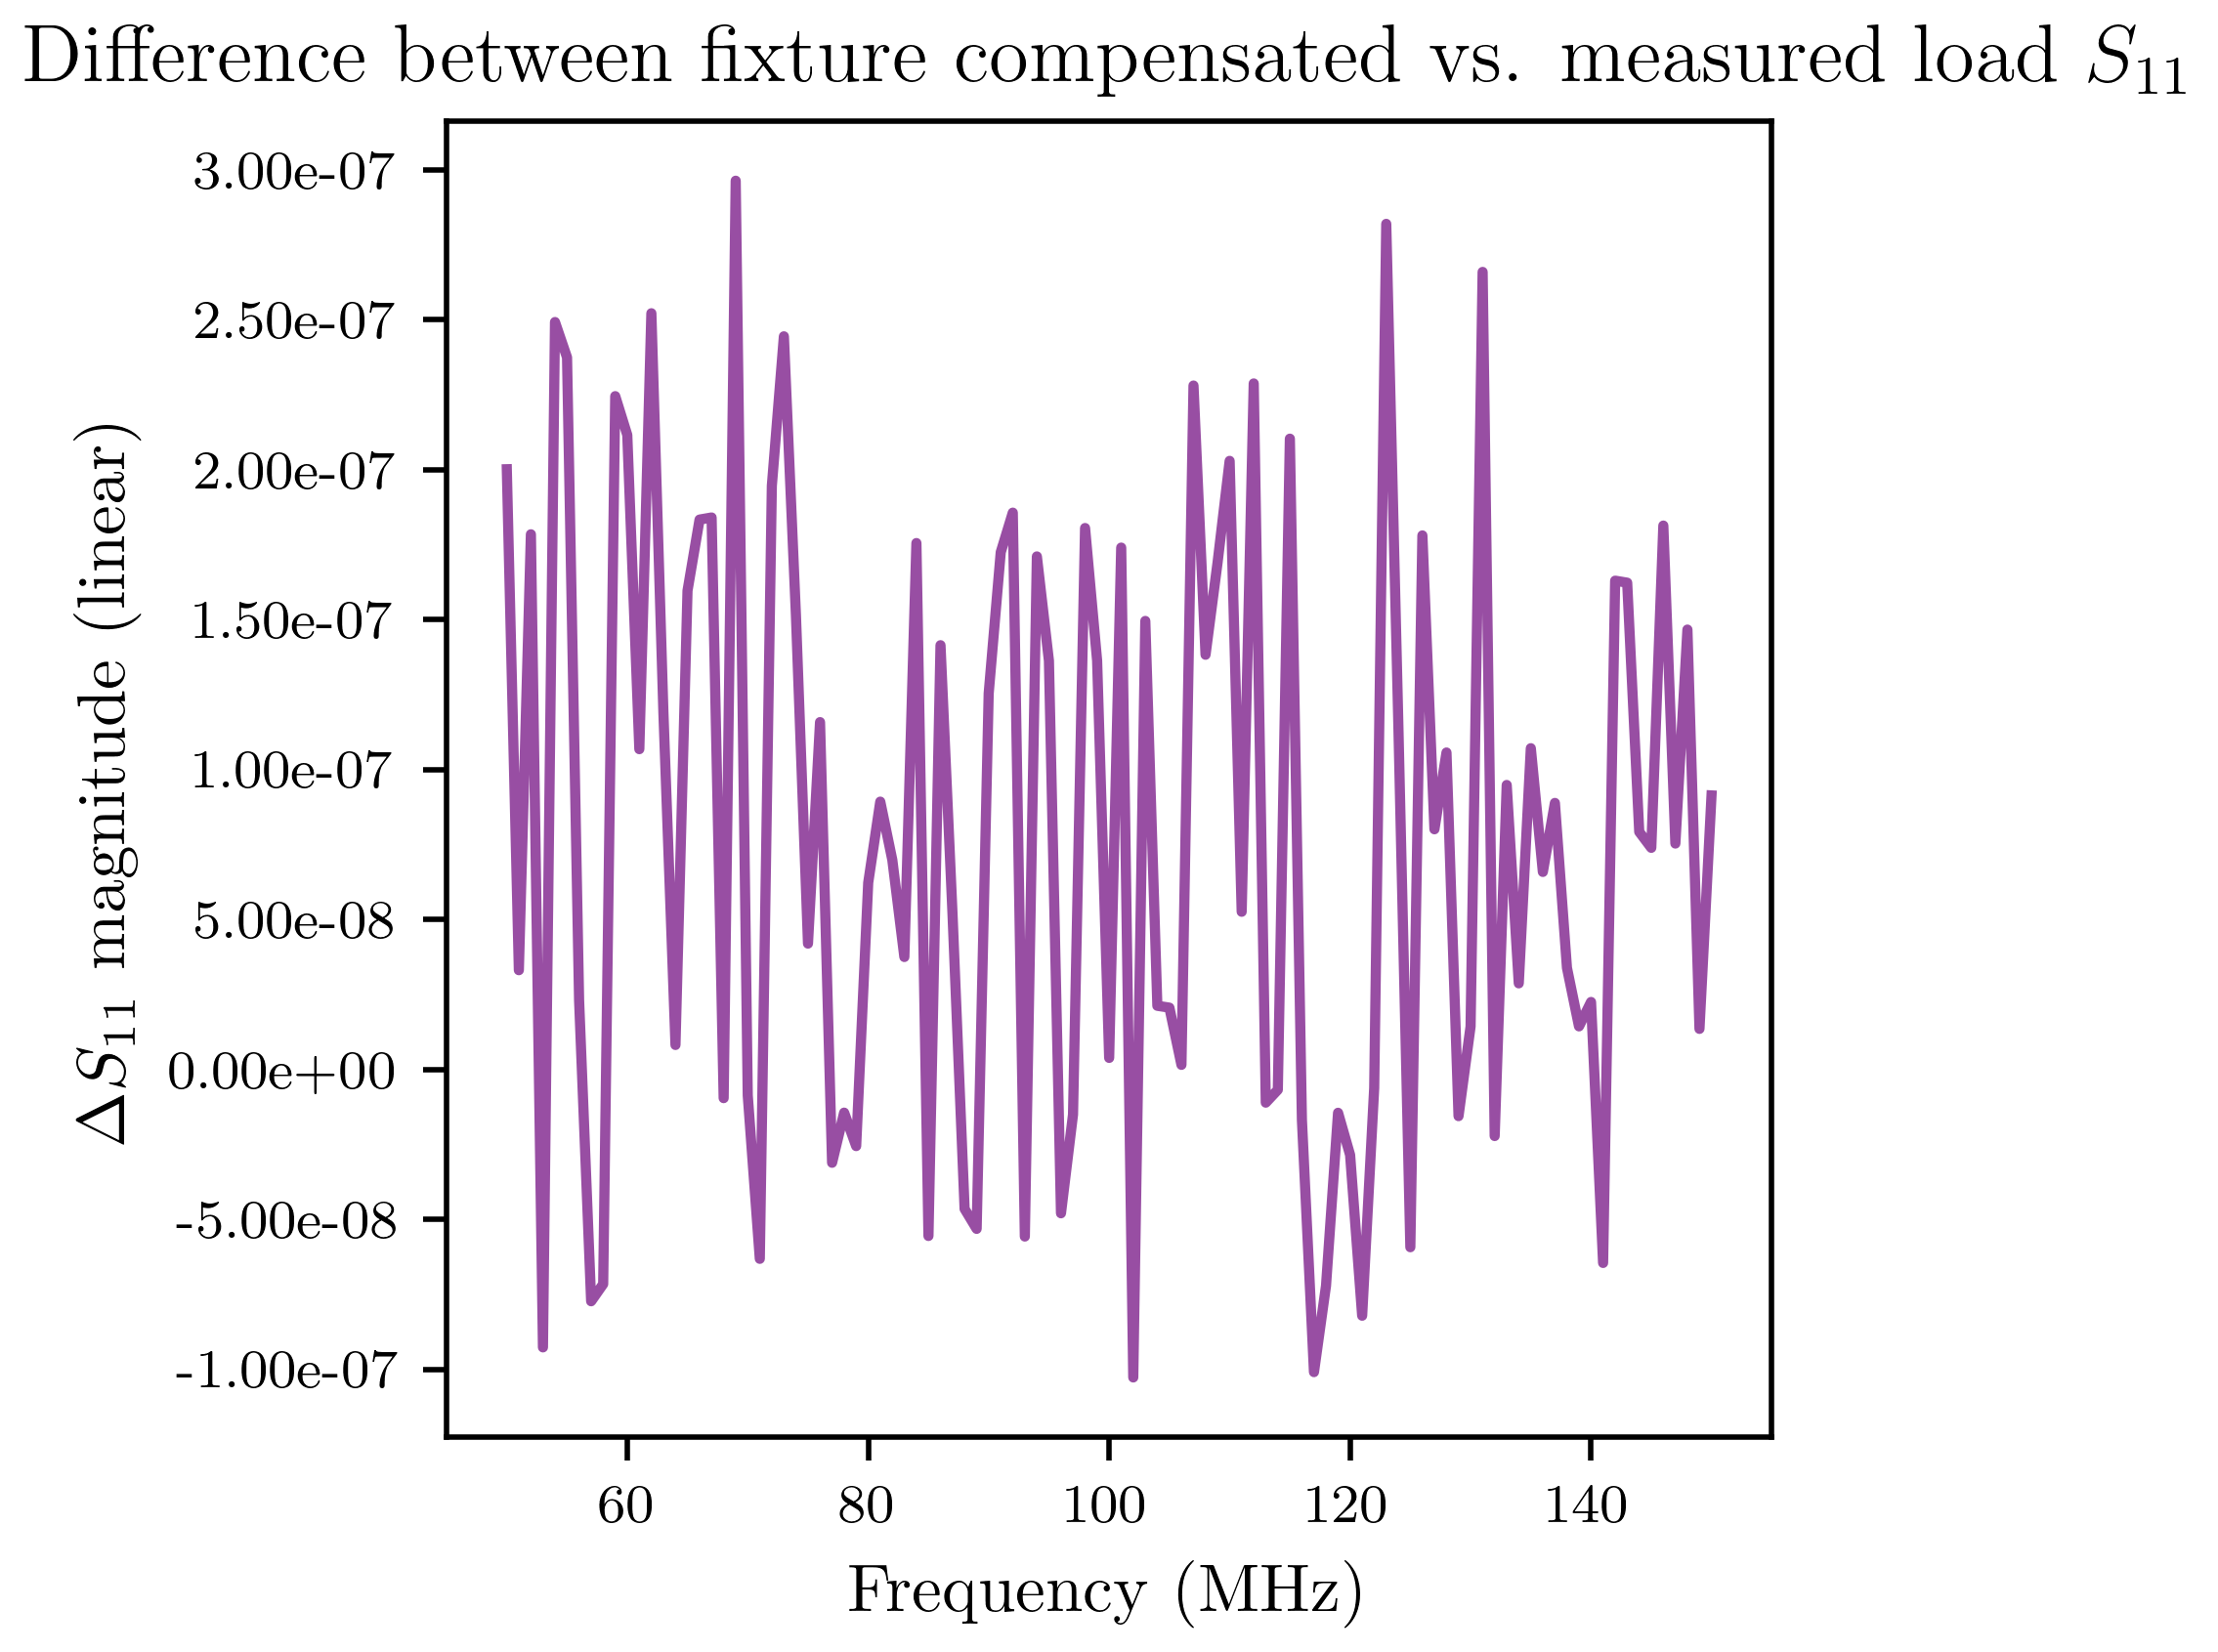
\includegraphics[width=.7\textwidth]{tparam}
    \caption{A plot comparing a simulated load and a model derived through fixture compensation. A load+cable configuration was simulated in the PathWave RF Synthesis software which was measured using the tools within the program. Measurements were then taken of the simulated cable on its own which were used to derive T-parameters and de-embed the cable from the fixture. The resulting model for the simulated load is shown in purple and plotted against the in-program measurement of the load shown in orange. We see that the model and measurement agree to within six decimal places. S-parameter magnitudes are shown on a linear scale and S-parameter measurements within the software were noiseless.}
    \label{fig:tparam}
\end{figure}


adding the path back in for the LNA measurements...